\documentclass[11pt,a4paper]{article}
\usepackage[margin=25mm]{geometry}
\usepackage[T1]{fontenc}
\usepackage{lmodern}
\usepackage{amsmath,amssymb,mathtools,amsthm}

\usepackage{booktabs,tabularx,longtable,array}
\usepackage{graphicx}
\usepackage[font=small,skip=7pt]{caption}
\usepackage{microtype}
\usepackage{enumitem}
\usepackage{xcolor}
\usepackage[colorlinks=true,urlcolor=blue,linkcolor=blue,citecolor=blue]{hyperref}
\setlength{\emergencystretch}{4em}
\setlength{\parskip}{0.45em}
\setlength{\parindent}{0pt}
\renewcommand{\baselinestretch}{1.12}
\widowpenalty=10000
\clubpenalty=10000
\displaywidowpenalty=10000
\setcounter{tocdepth}{3}
\newcolumntype{Y}{>{\raggedright\arraybackslash}X}
\newtheorem{proposition}{Proposition}
\newtheorem{definition}{Definition}
\newtheorem{remark}{Remark}
\newtheorem{example}{Example}
\DeclareMathOperator{\Var}{Var}
\DeclareMathOperator{\E}{E}
\newcommand{\ind}{\mathbf{1}}
\newcommand{\code}[1]{\texttt{#1}}
\newcommand{\artifactpath}[1]{\nolinkurl{#1}}

\hypersetup{pdftitle={Review Histories in Textbook Formalization},pdfsubject={Measurements, comparisons, and statistical analysis},pdfauthor={}}
\title{Review Histories in Textbook Formalization\\[0.6em]\large Measurements, Comparisons, and Statistical Analysis}
\author{}
\date{English edition -- Version 0.5.0\\6 September 2026}
\begin{document}
\maketitle
\begin{abstract}
A textbook formalization project repeatedly turns mathematical tasks into candidate Lean files, checks and reviews those submissions, and revises them in response to findings. Saved candidates, review inputs, judgments, and issue records make these decisions traceable and provide the material for this retrospective evaluation. The report explains how retained evidence becomes directed connections, how selected candidate revisions form continuous segments, and how failure-origin paths are observed until first recorded pass or exit. It then distinguishes the properties checked by an evaluator from conformity to the intended task, develops a four-cell candidate--criterion comparison, and derives limits from coarse measurements, missing information, and stopping rules. A historical definition witness and an exhaustive Boolean challenge demonstrate specific gaps between formal acceptance and task conformity. In the selected history, paired recorded acceptance increases on average across revisions, while later steps of the fixed failure-origin paths have a lower pass proportion than first steps. Task-weighted comparisons, paired t calculations, task-cluster resampling, an exact McNemar calculation, and a two-group process model retain their distinct outcomes and denominators. The report assumes calculus, probability, linear algebra, and basic statistical inference. Its conclusions describe the retained evidence under explicit assumptions; recorded acceptance is not an independent measure of mathematical correctness.
\end{abstract}
\clearpage
\begingroup
\small
\setlength{\parskip}{0pt}
\renewcommand{\baselinestretch}{1.0}\selectfont
\tableofcontents
\endgroup
\clearpage
\section{The work that produced the review history}
\label{sec:introduction}
\subsection{From a textbook task to a reviewed Lean file}
\label{subsec:workflow}
The project turns definitions, theorems, examples, and problems from a probability textbook into Lean files. Lean is a programming language with a system for checking formal proofs. For a particular textbook task, a writing agent works from the task text and relevant mathematical material, writes a candidate file, and checks whether it builds. A reviewing agent then examines the submitted version against the task and the supplied review instructions. It records a judgment and, where applicable, findings that the writer can use in a revision. The writer may submit another version, which can be checked and reviewed again.

The review asks more than whether the compiler accepted the file. It examines whether the formal definition or statement expresses the requested mathematics, whether the proof addresses the required argument, and whether the dependencies and assumptions meet the applicable rules. A failure can therefore lead to changes in the statement, proof, or supporting definitions. A later review can also revisit an already accepted file. These activities leave several kinds of evidence: task text, saved candidate versions, build results, review inputs and instructions, recorded judgments, and descriptions of issues.

Those records served the work before they served this study. A writer needs to know what to revise; a reviewer needs to know which version and which task are being checked; a later maintainer needs to understand why a result was accepted or reconsidered. Keeping earlier evidence makes it possible to connect a decision to the material available at the time. Retaining a rejected candidate or an old review does not imply that it remains the current result. The records also do not constitute a complete log of every edit or every model call.

This is the shared pattern supported by the retained workflow documents and historical artifacts. The archive also includes reviews of official outputs, external contributions, and multiple file representations of a review. Instructions, tools, and recording practices changed. We therefore do not assume that every historical record was produced by one uniform implementation of today's formalization system. Appendix~\ref{sec:sources} identifies the source material supporting this account.

\begin{figure}[htbp]
\centering\small
\fbox{\parbox{0.90\linewidth}{\textbf{Textbook task and context.} Select the mathematical statement, definition, or problem to formalize.}}
\par\smallskip $\downarrow$ \par\smallskip
\fbox{\parbox{0.90\linewidth}{\textbf{Candidate and build.} The writer submits a saved Lean version; the build checks its technical acceptance in an environment.}}
\par\smallskip $\downarrow$ \par\smallskip
\fbox{\parbox{0.90\linewidth}{\textbf{Review and next action.} The reviewer checks the submitted mathematics and records a judgment and findings. Revision returns to the candidate step; acceptance may be followed by landing or later review.}}
\caption{The recurring work pattern. Evidence is retained along the way. The diagram does not assert that every archived record traversed every box.}
\label{fig:work-pattern}
\end{figure}

\subsection{Why a change from fail to pass needs interpretation}
A submission raises distinct questions. Can the software process it? Does its proof obey the specified dependency rules? Does its formal statement express the intended mathematics? Their answers can differ. For example, a proof of ``if the conclusion holds, then the conclusion holds'' can be formally valid while leaving the original problem unsolved. Lean's documentation makes the same distinction between validating a proof and checking what its statement means\cite{leanvalidation}.

Now suppose that an earlier review rejects a candidate and a later one accepts it. The writer may have corrected a mathematical problem. But the requirement or the evidence available to the reviewer may also have changed, or an earlier issue may not have been noticed again. The two judgment labels alone do not distinguish these explanations. The history is worth studying precisely because it retains more than the final pass: it offers some evidence about the objects, checks, and intermediate outcomes behind that change.

\subsection{A second workflow: turning records into analysis data}
\label{subsec:analysis-workflow}
The study begins after the writing and reviewing have taken place. It first organizes the retained evidence, associates it with task and candidate identifiers, and records which review materials and context are available. It then takes the archive's specified within-task adjacent pairs, asks which pairs can be ordered in time, and classifies what activity each connection represents. A changed candidate, a rereview of an official file, and a second representation of the same review are kept distinct. Only after this classification can selected revision connections be joined into continuous histories.

Two historical questions follow. Pairing the endpoints of a selected revision lets us ask how the recorded judgment changed. Following a continuous history from an explicit failure lets us ask at which step a first pass was recorded, or where observation ended without one. These are different constructions from the same archive. Section~\ref{sec:materials} explains their units, selection rules, and counts before any statistical result is used.

The study also examines selected saved candidates with explicitly specified checks, alongside deliberately constructed comparisons and a small task whose inputs can all be tested. Those materials address a different question: what information can an evaluator supply about a candidate? Together the report studies:
\begin{enumerate}[leftmargin=*]
\item \textbf{Measurement:} What does a named check establish, and what does it leave unresolved?
\item \textbf{Comparison:} What changes when we compare two candidates under each of two stated criteria?
\item \textbf{Recorded process:} How do judgments change across selected revisions and along retained failure-origin histories?
\end{enumerate}
Statistics can describe the recorded decisions even when independent judgments of mathematical correctness are unavailable. Their interpretation must then remain about those decisions.

\subsection{How to read the report and find a definition}
The chapters retain a practical order: the objects and how they were selected; the evaluation quantities; the mathematical arguments; the executable evidence; the paired statistics; and the observed process. Definitions fix the objects and quantities used in each analysis; propositions state consequences of explicit assumptions. Illustrative examples explain a calculation and are not additional experiments.

Section~\ref{sec:materials} defines task, candidate, record, connection, and continuous segment. Section~\ref{sec:framework} introduces the score and the comparison of two candidates under two criteria, called a four-cell comparison. Section~\ref{sec:mathematics} gives the measurement, stopping, and identification arguments. Section~\ref{sec:audit} explains the saved executable checks. Sections~\ref{sec:statistics} and~\ref{sec:process} develop the paired and process statistics. Appendix~\ref{sec:definition-index} provides a topic index with page references; Appendix~\ref{sec:sources} maps the analysis to supplied files.

The report assumes basic calculus, probability, linear algebra, and statistical inference, including their standard notation. Project-specific terms and statistical constructions are introduced where needed. Each average identifies what receives weight, and each proportion identifies its denominator.

\section{From retained records to analysis units}
\label{sec:materials}
\subsection{Task, candidate, review record, and evidence signature}
\label{subsec:record-units}
A \emph{task} is one mathematical assignment, such as formalizing a specified definition or proving a specified theorem. A \emph{candidate} is a saved version submitted for that assignment. A task can have several candidates, and a candidate can be reviewed more than once. A \emph{review record} preserves a judgment about an object together with the available supporting evidence and context. The object may be a candidate or an official output.

The analysis identifies retained reviewer-produced evidence using an \emph{evidence signature}. Its curated main collection contains 3,231 such signatures. This is a count of evidence items under the archive's identification rules. It is neither a count of tasks nor a guarantee of 3,231 separate review executions. In particular, the raw and normalized result files from one review can survive as separate evidence items. A later classification recognizes some such relationships rather than interpreting them as repeated independent reviews.

\subsection{One task, three submissions, two connections, one segment}
\label{subsec:running-example}
Consider an illustrative theorem task with three submitted versions A, B, and C. Let their corresponding review records be $r_A,r_B,r_C$, with judgments fail, fail, pass. Suppose A-to-B and B-to-C both satisfy the candidate-revision rule defined below, and suppose the middle endpoint is exactly the same review record $r_B$ in the two connections. The task then supplies:
\begin{itemize}[leftmargin=*,nosep]
\item one task and three submitted candidate versions;
\item three review records in this illustration;
\item two directed \emph{connections}, also called \emph{edges}: $r_A\to r_B$ and $r_B\to r_C$;
\item one \emph{continuous segment}, formed by joining those two edges at $r_B$.
\end{itemize}
Thus two edges contain four endpoint occurrences, but only three distinct endpoint records. The repeated middle record matters both for reconstruction and for statistical dependence. A connection describes the relation between two retained observations; it does not count the edits or model calls between them.

Continuity requires the shared record, not merely the same task identifier or the same candidate text. Suppose a later version D appears after an official-output review, a connection that fails the chosen rule, or a gap with unresolved time order. We cannot extend this segment to D just because the task is unchanged. If D and a still later version E begin another eligible sequence, the same task contributes a second segment. Nothing in this construction asserts that the underlying work stopped during the gap.

The full segment and its observation for a particular question are also distinct. In the fail, fail, pass example, following the segment until its first pass uses both edges. In an illustrative fail, pass, fail segment, the full reconstruction can still contain two eligible edges, but a first-pass analysis uses only the first. It does not reinterpret the last failure as if it preceded that pass. These examples explain rules; they are not added observations.

\subsection{From evidence to 2,645 directed adjacent connections}
\label{subsec:adjacency}
To study what changed between reviews, the analysis starts with the archive's frozen within-task adjacency. It retains an original adjacent pair only when both endpoint signatures belong to the curated main collection. It does \emph{not} discard intermediate records and then connect whichever remaining records become neighbors. This preserves gaps in the retained history.

That membership rule yields 2,738 pairs. Of these, 93 have ambiguous time order under the declared timestamp rules, including tied times or insufficient precision. They remain undirected evidence and do not enter a before--after analysis. The other $2,738-93=2,645$ pairs supply directed connections. Their order is a documented proxy based on recorded time and identifiers, not evidence that one review caused the next event. The count cannot be obtained simply by subtracting a task count from 3,231, because the rule preserves original adjacency instead of rebuilding a gap-free chain after selection.

Even a directed connection need not describe revision. One endpoint may review a candidate and the next an official file with unchanged text. Both endpoints may review official outputs. A raw result file may be followed by the normalized representation of that same review. The next step therefore classifies the activity, using the reviewed object, primary Lean text, source, registered context, and prior structured findings. The pass/fail judgment itself is not used to assign the activity category.

\subsection{Which connections count as candidate revisions: 465 and 367}
\label{subsec:revision-rule}
The classifier applies rules in order. It first recognizes the two representations of the same review, then explicitly marked external reviews, then checks for distinct executions under the same registered conditions. Matching conditions without evidence of distinct executions remain unresolved. It next recognizes candidate landing into an official output with unchanged primary text. Only after those earlier cases have been handled does it assign \emph{candidate revision}: the later reviewed object must be a candidate, and the primary Lean text must differ between endpoints. Remaining official-to-official pairs become official rereviews; other unresolved pairs retain a mixed or unknown category.

Within candidate revision, \emph{high confidence} means the earlier review contains structured findings; without such findings, the connection has \emph{medium confidence}. These are reproducible rule labels, not numerical confidence levels or certifications that a mathematical problem was repaired. The rule detects a changed candidate following recorded issues; it does not independently establish that the change resolved those issues. The implementation calls this category \code{candidate\_repair}; this report uses ``candidate revision'' to keep that distinction explicit.

The resulting categories partition all directed connections:
\begin{table}[htbp]
\centering\small
\caption{Activity categories for the 2,645 directed connections. Counts are connections, not executions or tasks.}
\label{tab:roles}
\begin{tabularx}{\linewidth}{Y r Y}
\toprule
Category & Count & Interpretation \\
\midrule
Candidate revision & 465 & Changed primary text; later object is a candidate \\
Candidate landing & 241 & Candidate followed by official output with the same text \\
Official rereview & 1,176 & Both objects are official outputs \\
External review & 207 & Explicitly marked external-review source at an endpoint \\
Same review, two representations & 166 & Recognized raw and normalized result pair \\
Distinct, same-condition review & 0 & Requires explicit evidence of separate executions \\
Mixed or unknown & 390 & Available fields do not resolve the activity \\
\midrule
Total & 2,645 & Each connection is assigned once \\
\bottomrule
\end{tabularx}
\end{table}

The 465 candidate-revision edges concern 250 distinct tasks and divide into 367 high-confidence and 98 medium-confidence edges. The full 465-edge set supplies the paired revision analysis in Section~\ref{sec:statistics}. Its high-confidence sensitivity analysis uses the 367-edge subset, which represents 207 tasks. Task counts describe the distinct identifiers represented after a selection; unlike disjoint edge counts, they need not add across subsets because a task can contribute to both.

\subsection{Joining 367 edges into 262 full continuous segments}
\label{subsec:segment-rule}
For the process question, the reconstruction uses only the 367 high-confidence candidate-revision edges. Starting from an edge without an eligible predecessor, it appends an eligible next edge only when the earlier edge's later review identifier equals the next edge's earlier review identifier. It continues until there is no such edge. The result is a \emph{maximal continuous segment}: a chain that cannot be extended within this chosen edge set. The archived term is \emph{episode}; later chapters also call it a \emph{path} or \emph{process}.

This grouping assigns every selected edge once and produces 262 segments. It ends at an ineligible connection, an unresolved time-order boundary, or the end of observed connections. A recorded pass does not itself terminate this reconstruction: pass labels are used in the next analytical operation. Table~\ref{tab:segment-lengths} makes the edge-to-segment conversion checkable.

\begin{table}[htbp]
\centering\small
\caption{Lengths of the complete reconstructed segments, before selecting failure origins or stopping at first pass.}
\label{tab:segment-lengths}
\begin{tabular}{rrr}
\toprule
Edges per segment & Segments & Edges contributed \\
\midrule
1 & 212 & 212 \\
2 & 38 & 76 \\
3 & 1 & 3 \\
4 & 5 & 20 \\
5 & 3 & 15 \\
12 & 2 & 24 \\
17 & 1 & 17 \\
\midrule
Total & 262 & 367 \\
\bottomrule
\end{tabular}
\end{table}

The second column counts segments; the third counts their edges. The 262 segments retain the same 207 represented tasks as the 367 edges, because grouping alone removes no edge. Multiple segments from one task remain connected by their task identifier for statistical grouping, even though they remain separate paths in the reconstruction.

\subsection{Selecting 230 failure origins, then observing 329 steps}
\label{subsec:failure-cohort}
The process analysis asks what happens after an explicit recorded failure. It therefore selects the 230 segments whose first review says fail, excluding the other 32 from this question. These selected segments belong to 182 distinct tasks. Here 230 counts starting segments, while 182 counts the task identifiers represented by them. Neither is a number of independent review executions.

Within each selected segment, observation now stops at the first later review that records pass, or at the segment boundary if no pass appears. This second operation changes the observed length, not the already fixed segment membership. Applied to the selected segments, it yields 329 observed steps. Each step is one eligible edge and takes its outcome from that edge's later review. Across the 230 paths, 206 terminate at a first recorded pass and 24 reach the segment boundary without one. The original failure record is the starting condition, not an additional observed step.

Thus 329 is not the sum of all 367 reconstructed edges under another name: failure-origin selection and first-pass stopping intervene. Nor is $206/230$ a success fraction among 182 tasks, since one task can supply several paths. Section~\ref{sec:process} follows the changing step denominators and distinguishes path exit from permanent task failure.

\begin{table}[htbp]
\centering\small
\caption{The two historical analysis routes after activity classification. Each row states the operation and its unit.}
\label{tab:units}
\begin{tabularx}{\linewidth}{Y Y}
\toprule
Operation & Result and use \\
\midrule
Keep all candidate-revision connections & 465 edges, 250 tasks: paired recorded-label changes \\
Restrict those edges to high confidence & 367 edges, 207 tasks: paired sensitivity route and input to path construction \\
Join high-confidence edges at shared review endpoints & 262 full segments: continuity defined before outcome-based selection \\
Keep segments starting at explicit failure & 230 segments, 182 tasks: the fixed process cohort \\
Follow each selected segment to first pass or boundary & 329 steps; 206 pass endpoints and 24 exits \\
\bottomrule
\end{tabularx}
\end{table}

\subsection{Why the selected execution sample has 14 pairs}
\label{subsec:execution-sample}
The larger history describes recorded judgments. To examine what explicitly defined evaluators can establish about saved code, a separate, smaller selection takes candidate pairs from the revision material. It contains six development pairs and eight holdout pairs separated by task, for a total of 14 pairs and 28 candidate endpoints. The same task is not split across development and holdout. These are selection partitions in a retrospective study: prior exposure to parts of the archive prevents interpreting them as a fully blind, independently sampled experiment.

Each pair receives two assessments. One checks permitted axiom dependencies; the other checks the narrow requirement that a theorem must not directly assume its complete conclusion. Each assessment considers the two candidates under two stated criteria. Its four candidate--criterion combinations form a \emph{four-cell table}, defined and worked through in Section~\ref{subsec:four-cells}. There are therefore $14\times2=28$ historical tables, reusing the same 14 pairs. Their measurement outcomes are reported in Section~\ref{sec:audit}; no new executions were added in this edition.

\subsection{Constructed comparisons, a definition witness, and a Boolean task}
\label{subsec:constructed-materials}
The study also asks whether a comparison method behaves as intended under deliberately chosen patterns of observed and missing scores. Seven constructed tables serve this purpose. Together with the 28 historical tables, they give 35 tables for evaluating the comparison procedures. This total counts tables, not 35 independently sampled tasks. Section~\ref{sec:audit} explains the six diagnostic questions asked of each table.

A separate historical definition witness examines one task whose two candidates use different conventions for countability. Six proved propositions establish relations among those candidates, an explicit reference, and the empty set. They describe one case rather than six independent successes.

Finally, a finite Boolean task asks for the output to be true exactly when its two inputs differ. There are four possible input pairs, so a complete behavioral reference is available. Nine implementations were deliberately designed: three matching implementations, five mismatching implementations, and one compilation-failure control. Section~\ref{sec:measurement-classes} uses the eight executable implementations to derive a measurement limitation; Section~\ref{subsec:boolean-audit} gives the complete results. Nine implementations of this single task do not supply nine independently sampled mathematical tasks.

These materials have connected purposes but different denominators. The historical revision and path analyses describe selected records. The selected executions and constructed cases test particular checks or exhibit counterexamples. Their counts cannot be added into a common sample size or treated as independent replications of one statistical claim.

\section{Evaluation quantities and the four-cell comparison}
\label{sec:framework}

\subsection{Candidate, criterion, environment, and score}
\label{subsec:score}

Consider a program that should return true exactly when its two Boolean inputs differ. One candidate always returns false; another computes the required exclusive-or operation. Both may compile as Lean programs, but only the second gives the required answer on every input. A score is useful only after we specify which of these properties it measures.

Let $C$ denote the candidate: its saved code and the declaration selected for checking. A declaration is a named definition or theorem in that code; selecting it in advance fixes the object being assessed. Let $R$ denote the criterion, specifying the check and its acceptance rule, and let $E$ denote the environment, including the compiler, libraries, search paths, and execution settings. The \emph{evaluation procedure} $g$ applies $R$ to $C$ in $E$.

When a valid numerical measurement is available, we write its value as
\[
q=g(C,R;E).
\]
Thus $q$ is the score returned by the specified procedure. We hold the environment fixed in a comparison. The acceptance scores used here are dimensionless: $1$ means that the named check passed and $0$ that it failed. They are decisions of that check, not probabilities that the mathematics is correct.

To use $g$, we must supply the actual procedure, target, criterion, and evidence. The notation does not itself define a general measure of semantic correctness. We next describe the procedure implemented in the audit.

\subsection{Axiom-policy measurement and missing or invalid scores}
\label{subsec:measurement-status}

The released \code{evaluate\_sources.py} implements a narrow axiom-policy
check. It captures the source, appends commands for the already selected
declaration, runs the recorded Lean 4.31.0 compiler, and extracts two things:
the printed declaration type and its reported axiom dependencies. The type
describes the declaration's interface or proposition. The axiom list records
assumptions on which that declaration depends. These are useful observations,
but neither automatically states the intended task's meaning.

For this procedure, $R$ supplies a list of allowed axioms. The score is $1$
exactly when every extracted axiom is on that list, and $0$ when at least one
extracted axiom is forbidden. For example, a successfully extracted occurrence
of \code{sorryAx} receives $0$ under a policy that forbids it. An empty list of
dependencies passes such a policy; missing compiler output is not an empty
dependency list. Lean documents the distinction between proof validity and
the meaning of the statement proved. \cite{leanvalidation}

Before comparing scores, the implementation checks that the selected declarations have identical printed types under fixed printer settings. This establishes a conservative interface match. It leaves behavior open: both Boolean programs above can have type \code{Bool -> Bool -> Bool}. If the printed types differ, this implementation does not establish a numerical comparison, although another meaningful comparison may still be possible.

To check behavior, we could run both programs on all four input pairs and compare their outputs with the required truth table. The finite challenge reported below includes exactly this additional test. It supplies evidence that the axiom-policy check alone does not collect.

A check can also fail to produce a usable score. We therefore retain its measurement status:

\begin{description}[leftmargin=1.2em,style=nextline]
\item[Measured.] A value was obtained for the named check. A measured zero is
an actual rejection by that check.
\item[Not run, missing, or uncertain.] The intended question is meaningful,
but its answer was not obtained. Examples include an unavailable compiler,
missing source, a timeout, or failure to extract the selected declaration.
The narrow axiom check does not turn a compilation failure into an axiom-policy
rejection: it did not obtain the axiom measurement.
\item[Invalid or not applicable.] The proposed comparison lacks the required
meaning, or the criterion does not apply to the selected object. Treating such
a cell as an unknown number would already assume a comparison that has not
been justified.
\end{description}

Coding depends on the question. A study of compilation success could assign zero to a compilation failure; the axiom-policy check cannot do so when it has obtained no axiom measurement.

\subsection{Four cells, conditional differences, and interaction}
\label{subsec:four-cells}

We now hold one evaluator and environment fixed and compare two candidates
under two criteria. Let $C_0$ and $C_1$ are the two
candidates, and $R_0$ and $R_1$ the two criteria. Write
\[
q_{ij}=g(C_i,R_j;E),\qquad i,j\in\{0,1\}.
\]
The example below gives all four candidate--criterion scores.

The following is an \emph{illustrative calculation}, not another experiment.
Use the two Boolean programs described above: $C_0$ always returns false,
while $C_1$ returns true exactly when its inputs differ. Let $R_0$ test only
the input pair (false, false), whose required output is false. Let $R_1$ test
all four input pairs, whose required outputs in the order (false, false),
(false, true), (true, false), (true, true) are false, true, true, false.
In this example $g$ means ``run the inputs specified by the criterion and
award $1$ if all required outputs match, otherwise $0$.'' It is a behavioral
test procedure for this example, not the released axiom-only procedure.

\begin{center}
\begin{tabular}{lcc}
\toprule
Candidate & $R_0$: one input & $R_1$: all four inputs\\
\midrule
$C_0$: always false & $q_{00}=1$ & $q_{01}=0$\\
$C_1$: exclusive-or & $q_{10}=1$ & $q_{11}=1$\\
\bottomrule
\end{tabular}
\end{center}

First compare the candidates while keeping the criterion unchanged. Let
$D_{C\mid R_0}$ denote the second candidate's score minus the first
candidate's score under $R_0$. Define $D_{C\mid R_1}$ in
the same way under $R_1$. Reading down the two columns gives
\begin{align*}
D_{C\mid R_0}&=q_{10}-q_{00}=1-1=0,\\
D_{C\mid R_1}&=q_{11}-q_{01}=1-0=1.
\end{align*}
The one-input test cannot distinguish the programs. The four-input test can.
Thus a reported candidate difference depends on which test is held fixed.

Next compare the criteria while keeping the candidate unchanged. Reading
across each row gives
\begin{align*}
D_{R\mid C_0}&=q_{01}-q_{00}=0-1=-1,\\
D_{R\mid C_1}&=q_{11}-q_{10}=1-1=0.
\end{align*}
The expanded test rejects the defective program but leaves the correct program
accepted. The negative first difference describes a lower test score; it does
not mean that improving a criterion made the program itself worse. All four
differences have units of \emph{score points}. They are not percentages of
program quality.

A diagonal comparison instead changes both ingredients at once. Write
$\Delta$ for that change:
\[
\Delta=q_{11}-q_{00}=1-1=0.
\]
Looking only at these two acceptance labels would hide both the improved
program and the more demanding test. The \emph{interaction}, denoted $I$,
records how much the candidate contrast changes when the criterion changes:
\begin{align*}
I&=D_{C\mid R_1}-D_{C\mid R_0}=1-0=1\\
 &=q_{11}-q_{10}-q_{01}+q_{00}.
\end{align*}
Regrouping the same four terms also gives
$I=D_{R\mid C_1}-D_{R\mid C_0}$. Interaction here is an arithmetic
description of the table, not evidence about psychological cooperation or
a causal mechanism. These four conditional differences, the diagonal
difference, and the interaction are the audit's six diagnostic questions.

\subsection{The two-factor Shapley allocation}
\label{subsec:allocation}

There are two paths from the top-left cell to the bottom-right cell. We can
change the candidate first and then the criterion, or change the criterion
first and then the candidate. Either path's two differences add to $\Delta$.
If we choose to weight the two orders equally, the candidate receives the
average of its two conditional differences, and the criterion receives the
average of its two conditional differences. Denote these allocations by
$\phi_C$ and $\phi_R$:
\begin{align*}
\phi_C&=\tfrac12[(q_{10}-q_{00})+(q_{11}-q_{01})],\\
\phi_R&=\tfrac12[(q_{01}-q_{00})+(q_{11}-q_{10})].
\end{align*}
They are the standard two-factor Shapley allocation. \cite{shapley} In the
example, $\phi_C=(0+1)/2=1/2$ and $\phi_R=(-1+0)/2=-1/2$. Their sum is zero,
as the diagonal comparison requires. In general, cancellation of the middle
terms gives $\phi_C+\phi_R=q_{11}-q_{00}=\Delta$.

The allocation is in score points and depends on giving the two orders equal weight. It is a summary of the table, rather than a recovered causal contribution from history. The interaction is already included in the averages; adding it once more would break their sum identity.

\subsection{Historical review: observed labels and partly observed conditions}
\label{subsec:historical-model}

In the four-cell comparison, the procedure and criteria are specified. A historical review is less controlled: the archive may record a decision while preserving only part of the process that produced it. For a review event $e$, distinguish the following roles:
\begin{itemize}
\item $Y_e$ is the recorded outcome label, such as pass or fail. It is a
category until a particular numerical coding is stated.
\item $O_e$ is the object actually reviewed, including the candidate code
and relevant context.
\item $K_e$ is the effective criterion actually applied in that review.
\item $M_e$ is the review apparatus: for example, the reviewer or model,
prompt, tools, and operating settings.
\item $U_e$ collects remaining influences that this description does not
separately record. No probability distribution or independence assumption
is being assigned to it.
\end{itemize}
The conceptual expression
\[
Y_e=\psi(O_e,K_e,M_e,U_e)
\]
then says only that the outcome arises from those ingredients through some
review procedure, named $\psi$. Unlike a fitted regression equation,
it supplies no coefficients to estimate and no known rule for predicting
$Y_e$. The earlier notation used $C_e^*$ for the effective criterion and
$\varepsilon_e$ for remaining influences; $K_e$ and $U_e$ avoid confusing
that criterion with candidate $C$ in our four-cell table.

For example, a stored contract's hash identifies the saved text, but cannot establish how closely the reviewer followed it. The effective criterion may remain partly unknown. A changed label can likewise accompany changes to the candidate, expectations, or review procedure. The later process analysis studies the recorded sequence under explicit path rules; it does not identify those separate influences.

We can nevertheless ask what a specified measurement distinguishes, what follows from an explicit observation model, and which comparisons the available evidence determines.
\section{Mathematical analysis: what the evidence determines}
\label{sec:mathematics}

A measurement can answer some questions while leaving others open. We begin with a finite example in which two checks give identical results for programs with different behavior. This leads to a bound on the mistakes that any decision rule using those checks must make.

\subsection{Measurement classes and the finite error bound}
\label{sec:measurement-classes}

Begin with the retained finite Boolean challenge. It contained nine fixtures,
of which eight were executable and one did not compile. Among the eight
executable fixtures, three matched the specified output on every one of the
four input pairs and five did not. Yet all eight passed both the axiom-policy
gate and the printed-type gate. A gate is simply a check returning pass or
fail. Imagine now giving another decision rule only those two gate outputs,
with no code, candidate name, or behavior results. It sees exactly the same
input---two passes---for every fixture. A deterministic rule, meaning one
that always gives the same answer to the same input, must give all eight the
same decision.

If the rule calls all eight task-conforming, it makes five mistakes. If it
calls all eight nonconforming, it makes three. The better of these two choices
still makes three mistakes. No more elaborate arithmetic on the same two bits
can tell it which three programs were correct. The behavior check succeeds
in distinguishing them because it supplies another observation.

We can state this argument for any finite set. Let $\mathcal X$ be the set of
objects being checked and $n$ its number of objects, with $n>0$. A particular
object is called $x$. Let $Z(x)$ be the retained measurement for that object,
which may be a pair of gate outputs rather than a number. Let $T(x)$ be its
reference answer: $1$ for conformity to a specified task reference and $0$
for nonconformity. The letter $T$ here denotes a binary task answer, not a
waiting time. In this example the reference is the exhaustive four-input
check; this notation does not assert that an equally usable reference exists
for every historical task.

Group together objects with the same measurement value $z$. Within such a
group, write $n_{z0}$ for the number with reference answer $0$, and $n_{z1}$
for the number with reference answer $1$. These are counts of objects. Let
$\delta$ return either $0$ or $1$ using only $Z(x)$. It must answer
for every object. Define its finite-set error fraction as
\[
\operatorname{Err}_{\mathcal X}(\delta)
=\frac{\text{number of objects for which }\delta(Z(x))\ne T(x)}{n}.
\]
This is a dimensionless fraction of mistakes in this set, not yet a
population probability.

\begin{proposition}[Unavoidable mistakes when measurements merge different answers]
\label{prop:measurement}
Under the preceding assumptions, every deterministic decision rule using
only $Z$ satisfies
\[
\operatorname{Err}_{\mathcal X}(\delta)
\ \ge\ \frac{1}{n}\sum_z\min(n_{z0},n_{z1}).
\]
The sum runs over the distinct measurement values. Some such rule attains equality.
Consequently, zero mistakes are possible exactly when every measurement group
contains only one reference answer.
\end{proposition}

\begin{proof}
Fix one measurement group. Since the decision rule receives the same input
throughout that group, it must choose one answer for the whole group. Choosing
$0$ misclassifies its $n_{z1}$ conforming objects; choosing $1$ misclassifies
its $n_{z0}$ nonconforming objects. Therefore the smallest possible number of
mistakes in this group is the smaller count. Add those minimum counts over
the groups and divide by the total number of objects. Choosing the majority
answer separately in every group achieves the bound. A group's minimum is
zero precisely when one of its two counts is zero.
\end{proof}

For the eight executable fixtures there is just one group, with $n_{z0}=5$
and $n_{z1}=3$. Substitution gives
\[
\text{smallest possible error fraction}=\frac{\min(5,3)}8=\frac38.
\]
The interpretation ``both gates passed, therefore the task was met''
instead has error fraction $5/8$. Thus $5/8$ describes that particular
accept-all interpretation, while $3/8$ is a limitation of \emph{every forced
deterministic binary rule restricted to the same two gate outputs}. Neither
is a historical error-rate estimate, and neither has the denominator needed
for defect-detection sensitivity. The noncompiling ninth fixture is not
silently added to this eight-object calculation.

Allowing the rule to abstain changes the question: it could avoid all mistakes
by refusing every decision, so we must also report the fraction it answers.
Randomization cannot lower the minimum \emph{expected} error here. If it
chooses $1$ with probability $r$, where $0\le r\le1$, its expected number of
mistakes in the single group is $5r+3(1-r)=3+2r$, whose minimum is $3$.
Individual randomized runs need not equal their expectation. These remarks
explain why the assumptions ``deterministic'' and ``answers every object''
appear explicitly in the proposition.

\subsection{Why acceptance records alone do not identify accuracy}
\label{subsec:accuracy}

The previous result assumed that reference answers were available and showed
what a coarse measurement loses. A different difficulty arises when reference
answers are absent. Suppose, for illustration, that the only retained outcomes
for four records are accept, reject, accept, reject. If all four reference
answers agreed with those outcomes, the recorded decisions would be fully
accurate. If every reference answer disagreed, they would be entirely
inaccurate. Both hypothetical lists are compatible with the four observed
decisions \emph{when no additional evidence constrains the reference answers}.
We have not changed mathematical truth; we have exhibited what the supplied
records alone fail to settle.

In symbols, let $A$ denote a recorded binary acceptance decision and $T$ a
reference answer. Observing $A$ without information that constrains $T$ cannot
choose between the possibilities $T=A$ and $T=1-A$. Their fractions of correct
decisions differ. This is called \emph{nonidentification}: different answers
to the research question remain consistent with what was observed. In a
four-record example the possible accuracy fractions are multiples of $1/4$,
not every real number between zero and one. Source analysis, an explicit
task reference, or independent adjudication may eliminate these possibilities;
the limitation concerns the stated observation scheme.

Historical labels also need a clear coding rule. Coding only ``pass'' as $1$
and all other labels as $0$ measures recorded acceptance versus nonacceptance.
If the other labels include partial or inconclusive decisions, this coding
does not automatically measure reviewer error. An accuracy calculation among
decisive pass/fail reviews would use a different denominator and report the
omitted fraction separately.

\subsection{Stopping, observation eligibility, and path exit}
\label{sec:process-theory}

\subsubsection{From a reconstructed segment to an observed path}
A full segment connects records through the high-confidence candidate-revision edges of Section~\ref{subsec:segment-rule}. The observed path is the portion followed under the stopping rule of Section~\ref{subsec:failure-cohort}. One step is a transition between submitted versions, rather than an internal edit, a model call, or a fixed amount of time. The path is reconstructed from saved records, and one task can have several separate paths.

Suppose the recorded sequence is fail, fail, pass. Starting at the first failure, there are two steps, and observation stops at the pass. Three candidate records have thus supplied two transitions. The chain might instead end while its latest review is still nonpassing; we call this a \emph{path exit}. The task could continue elsewhere, so exit does not imply permanent failure. Section~\ref{sec:process} applies this observation rule to the history. We first examine its consequences in a simple probability model.

Throughout the model, success means a recorded pass. A \emph{nonpass} includes every other label, including partial or inconclusive judgments, whereas a failure-origin path must begin with an explicit failure label. These conventions concern the review record, rather than independently certified task conformity.

\subsubsection{Constant conditional pass probability and predictable observation}
Consider repeated tosses of a coin with head probability $p$, where $0<p<1$, stopping at the first head. If heads represents a recorded pass, this gives a model of successive submissions with a constant pass probability. Real submissions may improve and their review conditions may change; those possibilities are set aside in this illustrative model.

To express exactly what the calculation needs, let $j=1,2,\ldots$ denote a possible step. Write $H_{j-1}$ for all information available \emph{before the result of step $j$}: earlier candidates, earlier review outcomes, and any observation decision already made. Define the observation and acceptance indicators, and their cumulative counts:
\begin{center}
\begin{tabularx}{\linewidth}{lY}
\toprule
Symbol & Meaning for a single path \\
\midrule
$B_j$ & 1 if no previous step has passed and step $j$ is to be observed; 0 otherwise. \\
$A_j$ & 1 if the review at that step records a pass; 0 if it does not. Set it to 0 when $B_j=0$, merely to complete the notation. \\
$N_k=\sum_{j=1}^k B_j$ & Number of eligible steps actually observed through step $k$. \\
$D_k=\sum_{j=1}^k B_jA_j$ & Number of recorded passes among those steps. With first-pass stopping this is at most 1. \\
\bottomrule
\end{tabularx}
\end{center}

Saying that $B_j$ is known from $H_{j-1}$ means that we decide whether this observation belongs in the analysis without first seeing its outcome. This property is often called \emph{predictable observation}. It is not a prediction that the next candidate will pass. For example, ``continue after a failure and stop after a pass'' uses information already available. ``Retain this row only if the next review looks promising'' can use information that was not yet available and need not satisfy this condition.

For an eligible step, the constant-probability assumption is
\begin{equation}
 P(A_j=1\mid H_{j-1})=p\qquad\text{whenever }B_j=1.
 \label{eq:constant-conditional-pass}
\end{equation}
This requires the same conditional pass probability after every eligible past history; equality of pooled pass proportions is weaker. Equivalently, $E(A_j\mid H_{j-1})=p$ on eligible histories.

\begin{proposition}[A constant conditional probability under an explicit observation rule]
\label{prop:stopping}
Suppose observation eligibility $B_j$ is known before the step-$j$ outcome, and suppose equation~\eqref{eq:constant-conditional-pass} holds for every eligible history. For each fixed finite number $k$,
\begin{equation}
 E(D_k-pN_k)=0,\qquad\text{and hence}\qquad E(D_k)=pE(N_k).
 \label{eq:stopped-count-identity}
\end{equation}
If, in addition, the first step is observed and every nonpassing step is followed by another observed step until the first pass, the first-pass step $T$ satisfies
\begin{equation}
 P(T=j)=(1-p)^{j-1}p,\qquad j=1,2,\ldots.
 \label{eq:geometric-pass}
\end{equation}
\end{proposition}

\begin{proof}
At an eligible step the expected value of $A_j-p$, given the past, is $p-p=0$. At an ineligible step $B_j(A_j-p)=0$. Since eligibility is already known, both cases give
\[
 E\{B_j(A_j-p)\mid H_{j-1}\}=0.
\]
Averaging over the possible past histories still gives zero. Add this identity for the fixed set of steps $1,\ldots,k$. The sum inside the expectation is precisely $D_k-pN_k$, proving equation~\eqref{eq:stopped-count-identity}.

With observation continuing after every nonpass, a first pass at step $j$ requires $j-1$ consecutive nonpasses followed by a pass. Multiplying the successive conditional probabilities gives
\[
 \underbrace{(1-p)\cdots(1-p)}_{j-1\text{ nonpasses}}p.
\]
This is equation~\eqref{eq:geometric-pass}. It tends to put more weight on early steps because a later first pass requires surviving all the earlier nonpasses. The calculation uses the stated conditional probabilities; a separate independence assumption is not needed in addition to that full-history condition.
\end{proof}

Equation~\eqref{eq:geometric-pass} gives a geometric first-pass step $T$, distinct from the task-conformity reference $T(x)$. For $p=0.2$, the probabilities of first passing at steps 1, 2, and 3 are $0.2$, $0.8(0.2)=0.16$, and $0.8^2(0.2)=0.128$. Even though fewer paths remain eligible at each step, the chance of passing \emph{among paths still eligible} remains $0.2$ in this example. Thus a shrinking set of eligible paths does not, by itself, refute a constant-probability model. It also does not establish that such a model fits the historical archive.

\subsubsection{Martingale formulation}
\label{subsec:martingale}
Some earlier analyses used the word \emph{martingale}. Here it describes the running discrepancy
\[
 M_k=D_k-pN_k=\sum_{j=1}^k B_j(A_j-p).
\]
Given the available past, its next change has mean zero: $E(M_k\mid H_{k-1})=M_{k-1}$. That is the relevant mathematical property, already proved above. A filtration is simply the increasing family of information sets represented here by the histories $H_0,H_1,\ldots$. The martingale property is therefore another way to state the zero-mean increment calculation.

\subsubsection{Averages with a random denominator}
Equation~\eqref{eq:stopped-count-identity} concerns expected \emph{counts}. It does not say that $E(D_k/N_k)=p$, because the number of observed steps can itself depend on earlier outcomes. A short coin example makes the distinction visible. Take $p=1/2$, stop at the first pass, and observe at most two steps:
\begin{center}
\begin{tabular}{lrrrr}
\toprule
Observed sequence & Probability & $D_2$ & $N_2$ & $D_2/N_2$ \\
\midrule
Pass & $1/2$ & 1 & 1 & 1 \\
Nonpass, pass & $1/4$ & 1 & 2 & $1/2$ \\
Nonpass, nonpass & $1/4$ & 0 & 2 & 0 \\
\bottomrule
\end{tabular}
\end{center}
Here $E(D_2)=3/4$ and $E(N_2)=3/2$, so $E(D_2)/E(N_2)=1/2$. But the average of the final path proportions is $E(D_2/N_2)=1/2+1/8=5/8$. Fast successes contribute a ratio of 1 after only one observation. Exchanging ``take a ratio'' and ``take an expectation'' therefore changes the answer.

If observation instead continues without a step limit, use $D$ and $N$ for the \emph{total} pass count and observed-step count at the eventual stopping point; these differ from $D_k,N_k$, which count only through a fixed finite step $k$. Since $P(T>k)=(1-p)^k$ tends to zero, a first pass occurs with probability 1. Consequently, $D=1$ and $N=T$ with probability 1, and that probability-zero exception does not affect the following expectation. The same distinction has the exact expression
\[
 E(D/N)=\sum_{j=1}^{\infty}\frac{p(1-p)^{j-1}}{j}
 =\frac{-p\log p}{1-p}>p.
\]
Integrating the geometric series $\sum_{r=0}^{\infty}x^r=1/(1-x)$ from 0 to $1-p$ gives $\sum_{j\ge1}(1-p)^j/j=-\log p$. Also $-\log p=\int_p^1(1/u)\,du>1-p$ for $0<p<1$. This is a property of the illustrative model, not a correction formula applied to the historical data.

\subsubsection{Exit and selection of successful paths}
The no-exit coin model assumes that every nonpass is followed by another observation. Now suppose that after each nonpass a second independent coin determines whether the path continues. Let $a$ be its continuation probability, with $0\le a\le1$. All these continuation coins and acceptance coins are independent in this illustrative construction. The events after an eligible step are then:
\begin{center}
\begin{tabularx}{\linewidth}{Yl}
\toprule
What happens & Probability \\
\midrule
Record a pass and stop & $p$ \\
Record a nonpass and exit the path & $(1-p)(1-a)$ \\
Record a nonpass and observe another step & $(1-p)a$ \\
\bottomrule
\end{tabularx}
\end{center}
These probabilities add to 1. Give the third one the short name $b=(1-p)a$: it is the chance of both not passing now \emph{and} reaching the next observation. It is not the probability of a pass.

For a pass to be observed at step $j$, the first $j-1$ steps must each produce the third event, and step $j$ must pass. Hence
\[
 P(\text{pass at step }j\text{ before exit})=b^{j-1}p.
\]
The events for different $j$ cannot both occur. Summing their probabilities and using $1+b+b^2+\cdots=1/(1-b)$ gives
\begin{equation}
 s:=P(\text{pass before exit})=\frac{p}{1-b}.
 \label{eq:pass-before-exit}
\end{equation}
Here $s$ is a \emph{whole-path} probability; $p$ is a probability for one eligible step. They have different denominators and answer different questions.

Finally, suppose we discard all paths that exit without a pass and report only successful paths. If $J$ is the step of their recorded pass, ordinary conditional probability gives
\begin{equation}
 P(J=j\mid\text{pass before exit})
 =\frac{p b^{j-1}}{s}=(1-b)b^{j-1}.
 \label{eq:selected-success-time}
\end{equation}
This is another geometric distribution, but its parameter is $1-b=p+(1-p)(1-a)$, which exceeds $p$ if $a<1$. Successful-path selection favors shorter histories: to be a long successful path, a record must survive additional opportunities to exit. The faster-looking distribution does not demonstrate a higher per-step pass probability.

For a concrete identification problem, consider two possible mechanisms:
\begin{center}
\begin{tabular}{lrrrr}
\toprule
Mechanism & $p$ & $a$ & $b=(1-p)a$ & $s=p/(1-b)$ \\
\midrule
I & 0.2 & 0.5 & 0.4 & $1/3$ \\
II & 0.5 & 0.8 & 0.4 & $5/6$ \\
\bottomrule
\end{tabular}
\end{center}
Both give exactly the same successful-path step probabilities: $0.6$, $0.24$, $0.096$, and so on. Yet their eligible-step pass probabilities are $0.2$ and $0.5$. Looking only at successful-path lengths cannot distinguish these mechanisms. The overall pass fraction would distinguish them: if both $s$ and $b$ were known, equation~\eqref{eq:pass-before-exit} would give $p=s(1-b)$. The ambiguity comes from what was retained, not from a failure of probability arithmetic.

The three quantities now have distinct meanings: the pass rate at an eligible step, the outcome of a fixed path, and the length of a path selected because it passed. Applying the model to historical records would require checking its observation assumptions. A retrospective edge classification can use the next candidate or review, so reproducing that classification does not establish the before-outcome condition in Proposition~\ref{prop:stopping}. The empirical analysis below is consequently restricted to the retained paths and their observed associations.

\subsection{Partial tables and logical constraints}
\label{sec:feasible-tables}

Return to the four-cell table in Section~\ref{sec:framework}. Sometimes we
have measured only the second criterion's column. We may nevertheless know
something about the first column. For example, if one axiom policy allows a
subset of the axioms allowed by the other, passing the more restrictive policy
logically implies passing the more permissive one for the same extracted
declaration. The direction of this implication must be verified; calling a
policy ``new'' does not establish that it is stricter.

Assume for the following \emph{illustrative cases} that both scores are binary
and that acceptance under $R_1$ implies acceptance under $R_0$. In symbols,
\[
q_{i1}\le q_{i0}\qquad\text{for each candidate }i\in\{0,1\}.
\]
For zero-one scores this inequality means simply that a right-column $1$
requires a left-column $1$. It does not impose the reverse implication.

If the measured right column is $(1,1)$, the left column must be $(1,1)$ too.
The only permitted full table consists of four ones, so all six differences
are already zero. Actually running the two left-column checks could verify
the assumption or reveal a contradiction, but cannot give these differences
another value while the assumption and observations remain valid.

If instead the measured right column is $(0,0)$, each left-column value may
still be either zero or one. The four permitted completions are listed below.
Write $d=q_{10}-q_{00}$ for the candidate difference under $R_0$. Since the
right-column difference is zero, the definitions give $I=-d$ and
$\phi_C=d/2$.

\begin{center}
\begin{tabular}{ccccrrr}
\toprule
$q_{00}$ & $q_{10}$ & $q_{01}$ & $q_{11}$ & $d$ & $I$ & $\phi_C$\\
\midrule
0 & 0 & 0 & 0 & 0 & 0 & 0\\
0 & 1 & 0 & 0 & 1 & $-1$ & $1/2$\\
1 & 0 & 0 & 0 & $-1$ & 1 & $-1/2$\\
1 & 1 & 0 & 0 & 0 & 0 & 0\\
\bottomrule
\end{tabular}
\end{center}

Thus $d$ can take exactly the values $-1,0,1$. Its lower and upper bounds are
$-1$ and $1$, but $0.3$ is not possible in this binary example. Likewise,
$\phi_C$ can be $-1/2,0,1/2$. The output choices are linked: we cannot take
$d=1$ from one row and $I=1$ from another and claim they describe one table.
They must come from the same completion.

\subsection{Identification of a linear comparison}
\label{subsec:linear-identification}

Call $\mathcal F$ the collection of all full tables that agree with the
observed cells, the score's permitted values, and the verified logical rules.
Represent a table by the vector $q=(q_{00},q_{10},q_{01},q_{11})^{\top}$. Here $\mathcal F$ names a collection of
possible tables, not a probability distribution over them. Assume for now
that at least one table is possible.

Let $L(q)$ be a comparison calculated from a full table. For the comparisons
used here it is a weighted sum
\[
L(q)=a_{00}q_{00}+a_{10}q_{10}+a_{01}q_{01}+a_{11}q_{11},
\]
where $a=(a_{00},a_{10},a_{01},a_{11})^{\top}$ is a fixed weight vector, so $L(q)=a^{\top}q$. For example, the
candidate difference under $R_0$ uses weights $(-1,1,0,0)$. The output remains
in score points. Saying $L$ is \emph{uniquely determined}, or
\emph{point-identified}, means that every permitted table gives the same
answer.

\begin{proposition}[When the available information determines a comparison]
\label{prop:completion}
The comparison $L$ is uniquely determined exactly when $L(q)=L(q')$ for
every two permitted tables $q$ and $q'$ in $\mathcal F$. For a weighted sum,
this condition can be checked by verifying
\[
a_{00}(q_{00}-q'_{00})+a_{10}(q_{10}-q'_{10})
+a_{01}(q_{01}-q'_{01})+a_{11}(q_{11}-q'_{11})=0
\]
for every such pair. Further valid evidence can only remove permitted tables.
If it leaves at least one table, the greatest lower bound of the answers
cannot decrease and their least upper bound cannot increase. For a finite
list these bounds are simply its smallest and largest values.
\end{proposition}

\begin{proof}
If two permitted tables give different answers, the observations and rules
allow both answers, so there is no unique answer. If every permitted table
gives the same answer, that answer is forced. For a weighted sum, subtracting
$L(q')$ from $L(q)$ gives the displayed expression. Finally, removing choices
from a list cannot produce a new value below its previous minimum or above
its previous maximum. The same statement uses greatest lower and least upper
bounds when the permitted scores form an infinite set.
\end{proof}

In the four-row example, observing $q_{00}=0$ removes the last two rows. The
possible values of $d$ shrink from $\{-1,0,1\}$ to $\{0,1\}$. Also observing
$q_{10}=1$ leaves only the second row and determines $d=1$. This is additional
information. By contrast, computing $\phi_C=d/2$ from each of the original
four rows removes none of them. A useful summary need not be a new
observation. The two-factor allocation can aid explanation without supplying
a missing cell or a missing task reference.

If a measurement contradicts a claimed rule, there may be no permitted table
at all. For example, an assertion that the two criteria always give the same
score for a candidate conflicts with measured scores $0$ and $1$ for that
candidate. This calls for an inconsistency report, not an invented completion.
The release's consistency guard rejects this specific conflict. Invalid or
inapplicable comparisons likewise need their meaning repaired before we
enumerate numerical possibilities.

For meaningful but unknown cells, the released numerical core allows values
between $0$ and $1$ and calculates bounds over separate per-cell intervals.
Each cell receives its own permitted range, and the calculation allows any
combination of values from those ranges without expressing constraints
between cells. This does not assume that random variables are independent
in the probabilistic sense. These are bounds on missing information, not statistical confidence
intervals. If the score is actually binary, the exact attainable values may
be discrete as above. If additional relations connect the cells, separate
per-cell intervals may also allow impossible combinations and yield wider bounds than
necessary. The baseline code makes specific equality and binary-implication
deductions; it does not implement a general solver for every collection
$\mathcal F$. The proposition explains the reasoning principle rather than
claiming an unimplemented capability.

This distinction also clarifies the historical comparison: verified policy
implications already determine the accepted cases' missing policy cells,
while other configurations can benefit from measuring those cells. Equal
availability of the six specified diagnostics with and without an allocation
does not establish that allocation is universally useless. It reflects what
information those particular questions require.

\section{What the executable checks establish}
\label{sec:audit}
We now apply these distinctions to the 14 selected candidate pairs and the separately introduced constructed materials (Sections~\ref{subsec:execution-sample} and~\ref{subsec:constructed-materials}). Compilation and axiom checks establish properties of a formal file; the definition counterexample and Boolean challenge examine whether those properties suffice for the intended task.

\subsection{Compilation, target extraction, axioms, and task meaning}
\label{subsec:lean-checks}
A Lean file can contain many named definitions and theorems. The \emph{selected target} is the declaration chosen before evaluation. A successful proof of another theorem in that file cannot substitute for checking this target.

It is useful to distinguish four questions. First, does the file \emph{compile} in the recorded software environment? This checks that its syntax, names, types, and supplied proofs are accepted there. Second, is the selected target present and extractable? Third, on which \emph{axioms} does that declaration depend? An axiom is a proposition admitted as a starting assumption. Lean can report dependencies reached through other definitions and theorems, as well as direct dependencies. Fourth, does the accepted declaration express and satisfy the intended task? The first three checks provide evidence for the fourth, but do not settle it by themselves. In particular, the kernel checks a proof of the formal statement actually written, relative to its definitions and assumptions; interpreting that statement against the requested mathematics is a further step\cite{leanaxioms,leanvalidation}.

The historical execution used Lean 4.31.0, a 240-second limit per candidate, and two concurrent processes. It applied two experimental axiom policies. The first excludes \code{sorryAx}, the dependency associated with a placeholder that lets an unfinished proof remain in a Lean file. The second permits only \code{propext}, \code{Classical.choice}, and \code{Quot.sound}, three named foundational axioms on its allowed list. Passing either policy means passing that dependency rule. It does not mean that the theorem has the intended hypotheses or that a definition uses the intended convention. These two policies are experimental checks, not reconstructions of the complete old and new historical review instructions.

All 28 historical candidate versions were attempted: 17 compiled, 11 failed, and none timed out. Of the 17 successful files, 16 exposed their preselected targets; all 16 passed both policies. The remaining successful file, \code{ex\_3\_1\_2/from}, lacked the selected declaration, which was not replaced after seeing the result. Six candidate pairs consequently had complete four-cell axiom tables, each containing four ones. These results concern the recorded current environment. The complete original dependency environment was not reconstructed, so a present compilation failure is not proof of an original historical failure.

\subsection{A narrow check for assuming the conclusion}
\label{subsec:assumed-conclusion}
An accepted proof can establish a statement weaker than the task intended. For an elementary illustration, suppose the task is to prove that $x^2\geq 0$ for every real number $x$. A replacement statement saying ``if $x^2\geq 0$, then $x^2\geq 0$'' is easy to prove: its assumption already supplies its conclusion. The conditional statement is logically valid, but it does not establish the requested unconditional result. This is an explanatory example, not an additional historical observation.

The separate requirement subcheck asks whether the principal theorem directly assumes its \emph{complete conclusion} as a public hypothesis. A single AI assessor performed this narrow check. It does not detect every possible weakening of a statement or every indirect way of moving work into assumptions, and no independent expert reference was available. The 14 pairs supply $14\times4=56$ cells for this requirement assessment. Among them, 27 were measured, 23 were not applicable, four were uncertain, and two were invalid. Only six tables were complete and comparable. ``Not applicable'' means that this particular check does not apply; ``uncertain'' means that the evidence does not settle it; ``invalid'' means that the proposed assessment cannot be used as specified. None is silently turned into a measured failure. These counts describe where measurement was possible, not how often historical mathematics was correct.

\subsection{Four assessment methods and diagnostic availability}
\label{subsec:diagnostics}
For each candidate pair and pair of requirements, there are six diagnostic questions: how the candidate change looks under each of the two requirements; how the requirement change looks on each of the two candidates; the total change when both are changed; and whether the candidate contrast itself changes when the requirement changes. The final question is the interaction introduced in the mathematical framework.

The four methods differ in the information they may use. \emph{Historical labels} use the saved judgments, with abstention when their evaluator cannot be identified with the current one. \emph{Fixed $R_1$} checks both candidates under the second requirement, denoted $R_1$. \emph{Four cells} uses all four candidate--requirement combinations. \emph{Four cells plus Shapley} uses the same observations and additionally allocates the diagonal change by averaging the two change orders explained earlier.

The fixed-requirement method also receives verified equality of effective rules and valid logical implications. For example, if passing a stricter allowed-axiom list necessarily passes a looser one, an observed strict-policy pass implies a loose-policy pass without another execution. Such an entry is recorded as a deduction. Withholding it would unfairly make the four-cell method appear more informative.

\begin{table}[htbp]
\centering\small
\caption{Number of the six diagnostic questions with a justified single-number answer. The ``Slots'' column is the denominator for every method in that row.}
\label{tab:availability}
\begin{tabularx}{\linewidth}{Y r r r r r}
\toprule
Evidence group & Slots & Labels & Fixed $R_1$ & Four cells & + Shapley \\
\midrule
Constructed examples (7) & 42 & 4 & 17 & 26 & 26 \\
Axiom: development (6) & 36 & 0 & 13 & 13 & 13 \\
Axiom: holdout (8) & 48 & 0 & 27 & 27 & 27 \\
Requirement: development (6) & 36 & 0 & 12 & 12 & 12 \\
Requirement: holdout (8) & 48 & 0 & 25 & 25 & 25 \\
\bottomrule
\end{tabularx}
\end{table}

For example, the first row contains seven constructed tables, with six questions each: $7\times6=42$ possible answers. Its four-cell method supplies 26, not 26 correct judgments about 42 independently sampled tasks. The development rows use six historical pairs, giving $6\times6=36$ slots; the holdout rows use eight, giving $8\times6=48$. The axiom and requirement rows reuse those same historical pairs. Their slots must not be counted as independent samples. The zeros in the historical-label column mean that saved labels from a different evaluator cannot supply the stipulated current measurements; they do not mean that every saved label was wrong.

Four-cell access adds nine answers over fixed-$R_1$ access in the constructed examples and none in the historical groups. Shapley allocation adds no answerable question because it adds no observation. The constructed tables also have 26 assessable, previously handwritten reference answers, with no detected implementation discrepancy. Those references check arithmetic in designed cases; they are not independently adjudicated judgments of historical semantic correctness. The statistical interpretation of the historical zero differences is treated separately in this report.

\subsection{Why the empty set distinguishes two definitions}
\label{subsec:definition-witness}
Consider the historical task \code{def\_2\_1}. A \emph{bijection} between two sets pairs every member of either set with exactly one member of the other: no member is missed or duplicated. The natural numbers $\mathbb N=\{0,1,2,\ldots\}$ form an infinite set. A finite set cannot be paired bijectively with all of them. In particular, the empty set $\varnothing$, which has no members, cannot supply a partner for the natural number $0$.

Two conventions for ``countable'' are common. One includes finite sets together with sets that admit a bijection with $\mathbb N$; the other means specifically that a bijection with $\mathbb N$ exists. Both retained task texts use the second convention. The earlier candidate instead uses Lean's \code{A.Countable}, which includes finite sets. The later candidate uses the requested bijection convention and separately names the broader ``at most countable'' notion. The issue is fidelity to this task's stated convention, not a claim that the broader convention is generally wrong.

The audit's \emph{reference predicate} is the assertion ``there exists a bijection from $A$ to the whole set of natural numbers.'' Here $A$ is the set supplied to the definition. For readers checking the implementation, the reference is written in Lean as
\[
\code{Nonempty}\bigl(A\simeq(\code{Set.univ}:\code{Set}\ \mathbb N)\bigr).
\]
The symbol $\simeq$ requests a bijection; \code{Set.univ} denotes the whole set of elements of the indicated type, here the natural numbers; and \code{Nonempty} asserts that at least one such bijection exists. It does \emph{not} assert merely that $A$ has an element. Translating the task wording into this reference remains an inspectable AI interpretation made for the audit, without an independent expert reference; compilation alone does not certify that step.

The empty set now provides a complete argument that the older definition disagrees with the reference. The older predicate accepts it because it includes finite sets. The reference rejects it because a bijection would have to give $0$ a preimage in a set with no members. The newer definition rejects it for the same reason as the reference. A single counterexample suffices to refute a claim that two predicates agree for \emph{every} set.

The witness file retains both candidate bodies in separate namespaces, shares their common Mathlib import, and appends six proved propositions: the old predicate accepts the empty set; the reference rejects it; the new predicate rejects it; the new predicate agrees with the reference for every set; the old predicate does not agree universally with the reference; and the old and new predicates differ. Agreement of the new predicate with the reference follows by expanding their definitions. Six propositions describe one investigated case, not six independent successes.

The successful compilation exited with code zero in 217.685 seconds. Both candidate definitions had empty printed axiom sets; four witness propositions depended only on \code{Quot.sound}, and two had empty axiom sets. The source and message verifier passed 23 checks. An earlier Windows launcher failure caused by a long path occurred before compilation and remains archived; the successful run used a shorter directory. The result establishes this specific mathematical distinction relative to the chosen reference. It does not certify the entire revised file or all downstream theorems.

\subsection{Exhaustive behavior checks on one Boolean task}
\label{subsec:boolean-audit}
The finite challenge removes the need to interpret advanced mathematics. Its task is a function of two Boolean inputs, each either false or true. The output must be true when \emph{exactly one} input is true. Because there are $2\times2=4$ possible input pairs, the whole required behavior fits in Table~\ref{tab:truth-reference}. This reference was fixed before execution.

\begin{table}[htbp]
\centering\small
\caption{The complete reference for the two-input task.}
\label{tab:truth-reference}
\begin{tabularx}{\linewidth}{c c c Y}
\toprule
First input & Second input & Required output & Reason \\
\midrule
False & False & False & Neither input is true. \\
False & True  & True  & Exactly the second input is true. \\
True  & False & True  & Exactly the first input is true. \\
True  & True  & False & Two true inputs are not exactly one. \\
\bottomrule
\end{tabularx}
\end{table}

Nine implementations were deliberately designed: three correct versions, five incorrect versions with the same function type, and one compilation-failure control. A function type specifying two Boolean inputs and one Boolean output tells us what kinds of values may be supplied and returned. It does not tell us \emph{which} output is returned on a given input. Thus an ``always false'' function can have the same type as a correct exclusive-or function.

\begin{table}[htbp]
\centering\small
\caption{Saved observations on the finite task. All eight executable implementations passed both the axiom and printed-type checks. A dash means execution evidence was unavailable.}
\label{tab:finite}
\begin{tabularx}{\linewidth}{l Y c c}
\toprule
ID & Implementation & Mismatched inputs & Behavior \\
\midrule
01 & Exclusive-or & 0/4 & Match \\
02 & Boolean inequality & 0/4 & Match \\
03 & Conditional exclusive-or & 0/4 & Match \\
04 & Conjunction: both inputs true & 3/4 & Mismatch \\
05 & Disjunction: at least one input true & 1/4 & Mismatch \\
06 & Equality behind a helper & 4/4 & Mismatch \\
07 & Constant false & 2/4 & Mismatch \\
08 & First argument only & 2/4 & Mismatch \\
09 & Undefined function & -- & Uncertain \\
\bottomrule
\end{tabularx}
\end{table}

Table~\ref{tab:finite} compares each executable version with all four reference rows. For example, disjunction fails only when both inputs are true: it returns true while the task requires false. Exhaustive execution therefore identifies three matches and five mismatches; the unexecutable version remains uncertain. Passing the two preliminary checks is insufficient to establish the required behavior. Since these are nine designed implementations of \emph{one} task, the fraction five out of eight is not a population false-acceptance estimate or evidence from eight independently sampled tasks. Capability-oriented behavioral testing provides a methodological precedent\cite{checklist}; no NLP performance result from that work is transferred here. Finite execution also differs from the kernel-checked propositions in the definition example.

The original evaluator compiled a fixed correct baseline alongside each implementation, making 18 candidate compilations. Nine behavior-probe compilations brought the total to 27 attempts. The repeated baseline is instrumentation, not extra independent evidence. A separate verifier reconstructed the observations from saved standard output without calling the original scoring computation. It passed 166 checks after correcting a newline-normalization defect: its first nine fixture-hash failures reflected LF versus CRLF line endings. Both verifier versions and the failure report are preserved. Only fixture newlines are normalized; hashes of executed sources and probes remain exact. No experiment was rerun to replace the failed verification record.

\subsection{Reconstruction and rejection of contradictory inputs}
\label{subsec:reconstruction}
All 35 saved comparison tables were reconstructed exactly after timing was excluded. The earlier reconstruction suite passed 52 tests, while its provenance/accounting validator passed 6,093 checks over 227 read source snapshots. These results check reproducibility under the implemented rules, not independent semantic correctness.

The audit also found an input-consistency problem. Suppose the new candidate is said to face \emph{identical effective requirements} in both columns, but its measured entries are $q_{10}=0$ and $q_{11}=1$. Here the first entry is that candidate's result under the first requirement, and the second is its result under the second requirement. Identical deterministic checks on the same candidate should not produce both rejection and acceptance. The old baseline could infer a requirement contrast of zero from the identity declaration while direct subtraction gave $1-0=1$. The portable implementation now rejects the contradictory input before writing a result, rather than presenting both answers as valid.

Its 50 unit and regression tests are a separate suite from the earlier 52 reconstruction tests. The report retains that implementation and its 35 compatibility cases. This writing revision changes the explanation, not the recorded experiments, their outcomes, or the production formalization corpus.

\section{Paired statistics of recorded decisions}
\label{sec:statistics}

\subsection{Outcome definition: recorded pass}
\label{subsec:pass-coding}
Across the selected candidate revisions, how much more often was a pass recorded at the later endpoint? The larger archive allows us to answer this question by pairing each earlier record with its corresponding later record.

We use all 465 candidate-revision edges across 250 tasks, selected by the activity rule in Section~\ref{subsec:revision-rule}; the first-pass stopping rule is not applied to this paired analysis. Each edge compares two versions of the same assignment; a task can contribute several such comparisons. Thus the earlier and later records are paired observations, while the task is the unit used to group repeated observations.

We first translate the recorded labels into a numerical outcome. Write $A=1$ if a record says \code{pass}. Write $A=0$ for the explicitly recorded labels \code{fail}, \code{inconclusive}, and \code{partial}. Thus $A$ answers only ``Was a pass recorded?'' A zero is not a claim that the mathematics is wrong. In particular, an inconclusive review has not established mathematical failure. Missing or unrecognized labels are rejected by the analysis script rather than silently changed to zero. The original four categories are also retained in Table~\ref{tab:labels}.

For one edge, subtract its earlier value from its later value. A change $0\to1$ contributes $+1$, a change $1\to0$ contributes $-1$, and an unchanged binary value contributes $0$. None of these quantities measures semantic correctness: the outcome remains the recorded decision.

\subsection{Task-equal and edge-equal mean changes}
\label{subsec:task-weighting}
Consider the illustrative tasks in Table~\ref{tab:task-weights}. Task A passes after one selected change. Task B has three selected changes and passes only at the third. Both eventually pass, but the numbers of recorded edges differ.

\begin{table}[htbp]
\centering\small
\caption{Illustrative example only: one task can contribute more edges than another. The entries are binary recorded-pass values, not mathematical-quality scores.}
\label{tab:task-weights}
\begin{tabularx}{\linewidth}{l c Y c}
\toprule
Task & Edges & Earlier $\to$ later values & Mean edge difference \\
\midrule
A & 1 & $0\to1$ & $1$ \\
B & 3 & $0\to0$, $0\to0$, $0\to1$ & $1/3$ \\
\bottomrule
\end{tabularx}
\end{table}

Giving each task one vote yields $(1+1/3)/2=2/3$. Giving each edge one vote yields $(1+0+0+1)/4=1/2$. The answers differ because the second calculation gives Task B three times the weight of Task A. Neither arithmetic operation is wrong. They answer, respectively, ``What is the mean of the tasks' own mean changes?'' and ``What is the mean change across the recorded edges?'' Neither is the fraction of tasks that eventually pass; that fraction is $2/2$ in this example.

We now name the same ingredients for the real data. Let $S$ be the number of represented tasks ($S=250$ in the main route). The index $k$ names a task, from $1$ to $S$, and $n_k$ is its number of selected edges. Within task $k$, the index $e$ runs from $1$ to $n_k$. Write $A_{ke,0}$ and $A_{ke,1}$ for the earlier and later binary values. Define
\begin{equation}
\begin{split}
d_k&=\frac{1}{n_k}\sum_{e=1}^{n_k}(A_{ke,1}-A_{ke,0}),\\
\widehat\mu_{\mathrm{task}}&=\frac{1}{S}\sum_{k=1}^{S}d_k,
\qquad
\widehat\mu_{\mathrm{edge}}=\frac{\sum_{k=1}^{S}n_kd_k}{\sum_{k=1}^{S}n_k}.
\end{split}
\label{eq:paired-estimands}
\end{equation}
Here $d_k$ is a task's mean edge difference, $\widehat\mu_{\mathrm{task}}$ is the task-equal mean, and $\widehat\mu_{\mathrm{edge}}$ is the edge-equal mean. All three quantities are dimensionless differences on the zero--one scale. Multiply by 100 to report percentage points. A task's $d_k$ also equals its mean later-endpoint value minus its mean earlier-endpoint value. This is the pair of task-level means used below.

For the complete retained set, there are 118 earlier pass occurrences and 328 later pass occurrences. Therefore
\[
\widehat\mu_{\mathrm{edge}}=\frac{328-118}{465}
=\frac{210}{465}\approx0.451613,
\]
or 45.16 percentage points. Averaging the 250 task differences instead gives $\widehat\mu_{\mathrm{task}}=0.570909$, or 57.09 percentage points. These describe the specified archive and inclusion rules exactly, before any probability model is imposed; displayed decimals are rounded.

\subsection{Why 465 edges are not 465 independent observations}
\label{subsec:edge-dependence}
Consider a chain with recorded values $0\to0\to1$. Its two differences share the middle record: it is the later endpoint of one edge and the earlier endpoint of the next. More generally, if a chain has $m$ edges and successive values $a_0,a_1,\ldots,a_m$, then
\[
(a_1-a_0)+(a_2-a_1)+\cdots+(a_m-a_{m-1})=a_m-a_0.
\]
Every interior value cancels. A long chain can therefore supply many rows without supplying equally many independent observations of net change.

The retained graph has 930 endpoint occurrences but only 783 distinct endpoint records; 147 records appear in two edges. Its 318 maximal chains, formed from all 465 selected edges rather than the 367 high-confidence edges used for the 262 process segments, satisfy the cancellation identity, with total net difference 210. Further dependence can arise from common task difficulty, feedback, and review conditions. There are 103 tasks with multiple edges, a maximum of 26 edges in one task, and 14.41\% of all edges come from the five largest task groups. These graph chains are a diagnostic of this edge set, not a replacement definition of the failure-origin processes studied later.

We therefore summarize each task by its paired difference $d_k$ before calculating the t statistic, and resample entire tasks when constructing the reference intervals. This preserves dependence \emph{within} each task. It does not prove that different tasks are independent: tasks can still share reviewers, batches, mathematical dependencies, or changing rules.

\subsection{Paired t calculation and its reference assumptions}
\label{subsec:paired-t-explanation}
\subsubsection{Mean difference and standard error}
The conditional calculation uses the 250 task-level paired differences and an independent-task reference model for the same record-selection mechanism.

Let $D$ be a task difference in that reference population, with mean $\mu_D=E(D)$ and standard deviation $\sigma_d$. For the observed $d_1,\ldots,d_S$,
\[
s_d=\sqrt{\frac{1}{S-1}\sum_{k=1}^{S}(d_k-\widehat\mu_{\mathrm{task}})^2}.
\]
The observed sample standard deviation is $s_d=0.430341$, or 43.03 percentage points.

Under independent task differences with common variance $\sigma_d^2$,
\[
\operatorname{Var}\!\left(\frac{1}{S}\sum_{k=1}^{S}D_k\right)
=\frac{1}{S^2}\sum_{k=1}^{S}\sigma_d^2
=\frac{\sigma_d^2}{S}.
\]
The estimated standard error is
\[
\widehat{\mathrm{SE}}=\frac{s_d}{\sqrt S}
\approx\frac{0.430341}{\sqrt{250}}\approx0.027217.
\]
This is 2.72 percentage points under the task model. Cross-task dependence would add covariance terms, so the displayed division by $\sqrt{250}$ need not describe the mean's uncertainty in the actual archive.

\subsubsection{Null hypothesis and observed statistic}
The paired null is $H_0:\mu_D=0$ for the specified task population. The saved two-sided calculation is\cite{nistpaired,scipyttest}
\begin{equation}
t_{\mathrm{obs}}=\frac{\widehat\mu_{\mathrm{task}}-0}{s_d/\sqrt S}
\approx\frac{0.5709091575}{0.0272171622}\approx20.9761.
\label{eq:paired-t-worked}
\end{equation}
The pair consists of each task's later-endpoint mean and that same task's earlier-endpoint mean. Treating the earlier and later collections as independent samples would discard this pairing; the model is imposed on their differences.

\subsubsection{Reference distribution and scope}
For independent, identically distributed normal task differences with positive variance, the null reference is Student t with $S-1=249$ degrees of freedom.

The present task differences are bounded and take discrete values, so the exact normal-difference model does not literally hold. With 250 tasks, the reported Student calculation is used only as an exploratory large-sample reference under the additional independent-task model. In particular, a large number of tasks does not certify independence or validate the accuracy of an extremely small tail probability.

With $Z\sim t_{249}$, the nominal two-sided p-value is
\[
p_{\mathrm{ref}}=\Pr\{|Z|\geq |20.9761|\}
\approx5.87\times10^{-57}.
\]
This is a nominal tail probability under the reference model, whose relevance to this selected archive is unverified. Its small numerical value does not establish mathematical improvement.

\subsection{Task-cluster resampling and reference intervals}
\label{subsec:cluster-resampling}
To assess variation in the mix of represented tasks, the saved analysis uses a bootstrap with the \emph{entire task} as the sampling cluster\cite{scipybootstrap}. Each draw retains that task's selected paired edges together.

Each repetition draws $S$ task identifiers, uniformly and independently from the observed $S$ identifiers. Every selected task carries all its edges and both endpoints with it. We recompute the task-equal mean from the selected task differences. For the edge-equal mean we instead divide the selected tasks' combined net change by their combined number of edges; that denominator may change across repetitions.

The saved analysis uses 20,000 repetitions. Sorting the resulting values and taking the 2.5th and 97.5th percentiles gives the reported central 95\% percentile interval. For the full data, the task-equal interval is $[0.518357,0.624482]$, or $[51.84,62.45]$ percentage points. The edge-equal interval is $[38.63,52.12]$ percentage points. Reproducibility uses NumPy PCG64 with seed sequences $[20260906,r]$, where $r=0,1,2$ identifies the three analysis routes, and linear percentile interpolation.

These are \emph{reference} intervals because their usual 95\% coverage interpretation requires independent, sufficiently comparable tasks produced by the same history and inclusion mechanism. Those assumptions have not been established for this retrospective archive. The mean $0.570909$ is fixed once the 250 observed differences are given; the intervals describe hypothetical variation in which tasks are represented. Whole-task resampling retains within-task dependence but cannot repair selection bias, cross-task dependence, or the absence of a semantic outcome.

This differs from a \emph{logical completion bound}. Suppose, for illustration, that an earlier score is zero and a later score is unmeasured but must be zero or one. The difference can be zero or one, with sharp bounds $[0,1]$. These possibilities carry no assigned probabilities and no 95\% coverage claim. Measuring the missing score can resolve the ambiguity. The task bootstrap instead varies the hypothetical sample while using scores that are already known.

\subsection{Results under three selection rules}
\label{subsec:paired-results}
The main analysis and two sensitivity routes are shown in Tables~\ref{tab:paired-effects} and \ref{tab:paired-tests}. A sensitivity route changes an inclusion rule to show what answer that altered question produces. The three routes were declared before numerical estimation in the previous revision session, but the archive was already familiar. This is retrospective exploration, not prospective preregistration. All three unadjusted two-sided reference tests are reported; no route is selected because its p-value is smaller, and the pointwise intervals do not provide a simultaneous confidence guarantee for all routes.

\begin{table}[htbp]
\centering\small
\caption{Recorded-pass changes, in percentage points. Brackets contain 95\% task-cluster percentile reference intervals conditional on the task model. Changing the route changes the included edges and tasks.}
\label{tab:paired-effects}
\begin{tabularx}{\linewidth}{Y r r r}
\toprule
Route & Edges / tasks & Task-equal change & Edge-equal change \\
\midrule
All candidate-change edges & 465 / 250 & 57.09 [51.84, 62.45] & 45.16 [38.63, 52.12] \\
Both endpoints pass/fail & 440 / 236 & 55.73 [50.15, 61.21] & 44.09 [37.36, 51.18] \\
High-confidence edges & 367 / 207 & 76.93 [71.89, 81.73] & 59.95 [50.44, 70.10] \\
\bottomrule
\end{tabularx}
\end{table}

\begin{table}[htbp]
\centering\small
\caption{Paired calculations on task-level means. Before and after percentages are task-equal. Nominal p-values use an unverified Student-reference model and do not test semantic improvement.}
\label{tab:paired-tests}
\begin{tabularx}{\linewidth}{Y c c c}
\toprule
Route & Before $\to$ after & $t$ (df) & Two-sided $p_{\mathrm{ref}}$ \\
\midrule
All candidate-change edges & 29.16\% $\to$ 86.25\% & 20.9761 (249) & $5.87\times10^{-57}$ \\
Both endpoints pass/fail & 31.59\% $\to$ 87.32\% & 19.7176 (235) & $1.00\times10^{-51}$ \\
High-confidence edges & 6.92\% $\to$ 83.85\% & 30.5239 (206) & $2.21\times10^{-78}$ \\
\bottomrule
\end{tabularx}
\end{table}

In the full set, 182 task differences are positive, 67 are zero, and one is negative. There is actual variation, which makes the standard deviation nonzero and the t statistic calculable. The gap between task-equal and edge-equal means is also substantive: tasks with longer selected histories receive more weight in the second average and collectively have smaller net change per edge.

\begin{table}[htbp]
\centering\small
\caption{Original recorded verdicts for all 465 edges. Rows describe the earlier endpoint and columns the later endpoint. ``Inconclusive'' and ``partial'' remain visible even though neither is coded as a recorded pass.}
\label{tab:labels}
\begin{tabular}{lrrrr}
\toprule
Earlier / later & Pass & Fail & Inconclusive & Partial \\
\midrule
Pass & 105 & 12 & 1 & 0 \\
Fail & 206 & 117 & 5 & 1 \\
Inconclusive & 16 & 0 & 1 & 0 \\
Partial & 1 & 0 & 0 & 0 \\
\bottomrule
\end{tabular}
\end{table}

The four-category table explains why coding matters. Twenty-five edges have an inconclusive or partial endpoint. Seventeen move from such a result to pass, and one moves from pass to such a result. The main average therefore includes changes in whether a decisive pass was recorded. Restricting both endpoints to pass/fail removes these edges but also changes the represented tasks. It is a different selected target, not the same sample with a better name.

The high-confidence route uses the inherited confidence classification of candidate-change edges; ``high confidence'' is not an independent certification of mathematical repair. The rule uses prior structured findings. A descriptive check added after the main estimates shows markedly different starting compositions: the high-confidence subset starts with 21 passes among 367 edges, while the 98-edge medium-confidence complement starts with 97 passes and ends with 87. The complement spans 81 tasks, with task-equal change $-11.73$ percentage points and edge-equal change $-10.20$. No new test or interval is attached to that post-estimation check. A group beginning almost entirely at pass has little room to increase, whereas a group beginning mostly without pass has much more room. Thus the larger high-confidence change does not establish that its revisions are more effective.

Other explanations remain unresolved. The source-review contract fields differ on 45 edges and task-content fields on two; matching fields do not prove identical effective review conditions. Of 783 unique endpoint records, 781 have unknown check extent, one explicitly reports no review, and one a reviewability block. Independent execution was not checked by this projection. There are 451 edges outside the separate case assessment, so the larger statistical set lacks a corresponding semantic assessment for those edges. Candidate improvement, changed assessment conditions, and selective continuation can all produce recorded-label movement. Regression to the mean may also contribute. Without an appropriate comparison design and independent semantic outcome, these explanations cannot be separated by a small p-value.

\subsection{Why zero diagnostic differences give an undefined t statistic}
\label{subsec:zero-differences}
The smaller evaluator comparison measures a different outcome: the \emph{number of prespecified diagnostic questions with a definite answer}. The four-cell method is compared with a baseline that checks both candidates under $R_1$ and also uses verified relationships between the criteria. Those deductions are part of the baseline's information.

For task $k$, let $C_{k,4}$ be the number of definite answers supplied by the four-cell method and $C_{k,F}$ the corresponding number supplied by this fixed-requirement baseline. Each count lies from zero to six. Define $D_k=C_{k,4}-C_{k,F}$, measured in \emph{diagnostic questions}, not percentage points. In each of the two historical assessments, all 14 values of $D_k$ are zero; the individual answers also agree. Applying the same recipe gives
\[
\overline D=0,\qquad
s_D=\sqrt{\frac{1}{13}\sum_{k=1}^{14}(D_k-\overline D)^2}=0,
\qquad t_{\mathrm{obs}}=\frac{0}{0/\sqrt{14}}=\frac{0}{0}.
\]
The statistic is undefined, not a t-test result of $t=0,p=1$. The 250-task calculation above had nonzero variation and hence a defined denominator; this comparison has none.

The exact descriptive finding remains useful: these methods gave the same answers on these selected historical cases. But a task bootstrap would only redraw zeros, and a sign comparison would have no positive or negative differences to compare. Such calculations cannot reveal whether unobserved tasks would differ. Repeating the same 14 tasks in two assessments, or counting their six questions and four cells separately, does not create independent task information. Claiming population equivalence would require a defined population, a defensible uncertainty model, and a substantively acceptable difference specified for an equivalence question.

The seven constructed examples have fixed-baseline gains $[5,0,4,0,0,0,0]$. They demonstrate that additional information \emph{can} help; their deliberately chosen mixture does not estimate how often that happens in ordinary tasks. Shapley scoring adds no diagnostic availability beyond direct four-cell access in all 35 tables, consistent with its use of the same observations. These are different comparisons and should not be combined into a single claim of zero gains everywhere.

\subsection{The eight-pair compilation comparison: exact McNemar test}
\label{subsec:mcnemar}
There is a separate calculable comparison for the eight task-isolated holdout pairs: did the earlier and later candidates compile in the current test environment? Table~\ref{tab:compile-pairs} shows the complete paired observations. This outcome concerns compilation, not whether the intended mathematical statement was correctly represented.

\begin{table}[htbp]
\centering\small
\caption{Actual compilation outcomes for the eight holdout task pairs. The two off-diagonal cells, not the 16 endpoints treated separately, supply the directional information.}
\label{tab:compile-pairs}
\begin{tabular}{lrrr}
\toprule
Earlier / later & Fails & Compiles & Total \\
\midrule
Fails & 1 & 1 & 2 \\
Compiles & 1 & 5 & 6 \\
\midrule
Total & 2 & 6 & 8 \\
\bottomrule
\end{tabular}
\end{table}

Five pairs compile on both sides and one on neither. One changes from failure to success and one from success to failure. Each side therefore has six compiling candidates out of eight, giving the paired net difference $(1-1)/8=0$. The improving task is \code{def\_13\_2}; the declining task is \code{prob\_10\_1}.

The exact McNemar calculation asks whether discordant directions are balanced\cite{nistmcnemar}. Let $b=1$ count failure-to-success changes, $c=1$ the reverse changes, and $m=b+c=2$ the number of discordant pairs. Under a conditional null that the independent discordant directions are equally likely, the number $B$ of improving directions in a hypothetical repetition has a binomial distribution with $m=2$ trials and success probability $1/2$. Using twice the smaller tail probability, capped at one, gives
\[
p=\min\{1,\,2\Pr(B\leq1)\}
=\min\{1,\,2(1/4+1/2)\}=1.
\]
This p-value is a defined result with only two informative directions. It provides no directional evidence against that null; it does not prove equivalent compilation probabilities, absence of a revision effect, or semantic correctness. The holdout selection was stratified and retrospective, and task isolation does not itself prove statistical independence or erase prior exposure. The test is a limited illustration of a suitable paired-binary calculation, not a substitute for the larger task-level analysis.

Paired differences summarize selected revisions. To study their order, we next follow the steps of a path until its first recorded pass or its exit.
\section{Following the fixed failure-origin paths}
\label{sec:process}

\subsection{The fixed cohort, first-pass stopping, and exit}
\label{subsec:process-cohort}
We return to the high-confidence reconstruction defined in Sections~\ref{subsec:segment-rule} and~\ref{subsec:failure-cohort}. Its 367 edges form 262 full continuous segments. Selecting the 230 segments with an explicit failure at their origin gives the fixed cohort of 182 tasks. Selecting origins and stopping observation at first pass are separate operations; later records are never appended solely because they belong to the same task.

As defined in Section~\ref{sec:process-theory}, step 1 is the first eligible transition from the failing origin to another submitted candidate. Its outcome is the later candidate's recorded review decision. Each subsequent step is another such submitted-version transition. A path stops at its first recorded pass or at the end of the permitted chain, whichever comes first. The 230 paths contribute 329 observed steps in total. A row containing one such step and its outcome is called an \emph{eligible-step row}, traditionally a \emph{risk row}. ``At risk'' here means still eligible to record a \emph{first} pass.

There are two terminal outcomes. A total of 206 paths record a pass before the chain ends. The other 24 reach the chain boundary without such a pass. For this question, exit is an observed endpoint, not an unknown outcome silently assigned a failure label. It describes where this analytical path ends. It does not establish that the task was abandoned, that all future submissions would fail, or that an eventual pass elsewhere should be added to this path.

Changing the question changes the treatment of exits. If we asked how long the task would take to pass \emph{if the same mechanism continued indefinitely}, the post-exit outcomes would be unobserved. Calling those observations censored would not make the missing continuation known: additional assumptions would be needed to relate it to the observed paths. We do not estimate that hypothetical waiting time.

\subsection{Step counts, risk sets, and cumulative proportions}
\label{subsec:risk-counts}
At step 1 all 230 failure-origin paths are eligible. Of them, 167 pass, 18 end without a pass, and 45 continue to step 2:
\[
230=167+18+45.
\]
At step 2 only those 45 continuing paths remain. There are 29 passes, 4 exits, and 12 further continuations:
\[
45=29+4+12.
\]
The second denominator is 45 because we are asking about paths that reach step 2. It is not another sample of 230 paths, and it is not a comparison of all tasks before and after one extra revision. Table~\ref{tab:process-counts} shows the same accounting through the final observed step.

\begin{table}[htbp]
\centering
\caption{The fixed 230-path cohort. Each row partitions the paths observed at that step into pass, exit, or continuation.}
\label{tab:process-counts}
\small
\begin{tabular}{rrrrr}
\toprule
Step & Eligible & Pass & Exit & Continue \\
\midrule
1 & 230 & 167 & 18 & 45 \\
2 & 45 & 29 & 4 & 12 \\
3 & 12 & 1 & 0 & 11 \\
4 & 11 & 5 & 0 & 6 \\
5 & 6 & 2 & 1 & 3 \\
6 & 3 & 0 & 0 & 3 \\
7 & 3 & 0 & 0 & 3 \\
8 & 3 & 0 & 0 & 3 \\
9 & 3 & 0 & 0 & 3 \\
10 & 3 & 0 & 0 & 3 \\
11 & 3 & 1 & 0 & 2 \\
12 & 2 & 1 & 0 & 1 \\
13 & 1 & 0 & 0 & 1 \\
14 & 1 & 0 & 0 & 1 \\
15 & 1 & 0 & 0 & 1 \\
16 & 1 & 0 & 0 & 1 \\
17 & 1 & 0 & 1 & 0 \\
\midrule
Sum across steps & 329 & 206 & 24 & --- \\
\bottomrule
\end{tabular}
\end{table}

To write this bookkeeping once for all steps, let $n_j$ be the eligible count at step $j$, $d_j$ the passes at that step, and $c_j$ the exits after a nonpassing step. Then
\begin{equation}
 n_j=d_j+c_j+n_{j+1}.
 \label{eq:cohort-conservation}
\end{equation}
This is a counting identity, not a fitted model. The set of $n_j$ paths is the step-$j$ \emph{risk set}. Its decline is explained by the recorded pass and exit counts, without assuming a constant pass probability.

Two useful cumulative quantities keep the \emph{original} denominator 230:
\begin{align}
 F_P(j)&=\frac{d_1+\cdots+d_j}{230},
 &F_X(j)&=\frac{c_1+\cdots+c_j}{230}.
 \label{eq:finite-incidences}
\end{align}
$F_P(j)$ is the fraction of original paths that have passed by step $j$; $F_X(j)$ is the fraction that have exited without a pass by that step. The letters $P$ and $X$ stand for pass and exit. These are cumulative proportions, also called cumulative incidences. The remaining fraction is $n_{j+1}/230$, so the three fractions add to 1. At the last observed step,
\[
 F_P(17)=206/230=89.57\%,\qquad
 F_X(17)=24/230=10.43\%.
\]
Because exit is one of the two recorded terminal outcomes, calculating these finite-path proportions requires no assumption that exits are independent of future success.

Let a path's \emph{observed length} be its number of eligible transitions up to pass or exit. Adding those lengths gives 329. Their mean is therefore $329/230=1.4304$ transitions per path. A short path can end either in a pass or in an exit, so this is not the mean number of edits required for eventual success.

\subsection{First-step and later-step proportions have different composition}
\label{subsec:first-later}
All first steps together give $167/230=72.61\%$ recorded passes. All steps with index 2 or greater together give $39/99=39.39\%$. The denominator 99 is the sum of the later eligible counts in Table~\ref{tab:process-counts}, not 99 distinct paths or 99 independent tasks. A long path contributes several later rows. The difference ``later minus first'' is
\[
100\left(\frac{39}{99}-\frac{167}{230}\right)=-33.21
\quad\text{percentage points}.
\]
This is a description of two groups of observed rows. It is not the change that would occur if each of the same tasks were forced to receive exactly one more revision.

To show how these summaries vary under a reference sampling model, we resampled 182 entire tasks, with replacement, 20,000 times using the fixed seed 20260906. Whenever a task was selected, all its original paths and eligible rows were retained together. Each replicate recomputed the relevant ratio from pooled counts. The 2.5th and 97.5th percentiles of those results form the 95\% task-cluster reference intervals in Table~\ref{tab:process-estimates}. This preserves dependence within a task during resampling. It does not establish independence between tasks or adjust the observed history for selection. The interpretation of these reference intervals is explained in Section~\ref{subsec:cluster-resampling}.

\begin{table}[htbp]
\centering
\caption{Observed summaries and 95\% whole-task percentile reference intervals. Percentage-point differences use subtraction of proportions; observed length is measured in submitted-version transitions.}
\label{tab:process-estimates}
\small
\begin{tabularx}{\linewidth}{Yrr}
\toprule
Quantity & Estimate & Reference interval \\
\midrule
First-step pass proportion & $72.61\%$ & $[66.40,78.60]\%$ \\
Later-step pass proportion & $39.39\%$ & $[24.84,65.71]\%$ \\
Later minus first, percentage points & $-33.21$ & $[-48.39,-7.49]$ \\
Pass before fixed-path exit & $89.57\%$ & $[85.40,93.53]\%$ \\
Mean observed length to pass or exit & $1.4304$ & $[1.2271,1.6955]$ \\
\bottomrule
\end{tabularx}
\end{table}

These are ratios of pooled task totals, not means that give every task equal weight irrespective of its number of paths or rows. They therefore differ in weighting from the task-equal edge analysis in Section~\ref{sec:statistics}. The later-step interval is wide because the later rows are limited and unevenly distributed across tasks. For the already enumerated archive, the displayed proportions themselves are exact descriptions up to rounding; the intervals concern a hypothetical repetition under independent, exchangeable tasks with the same record-selection mechanism. Those assumptions have not been established by this archive.

\begin{figure}[htbp]
\centering
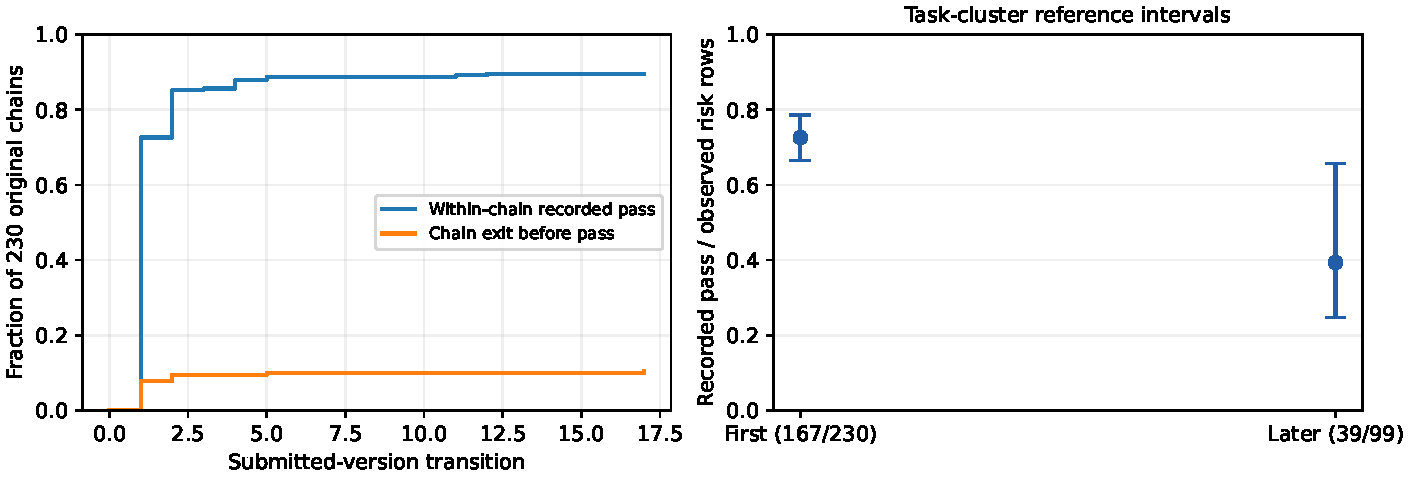
\includegraphics[width=\linewidth]{../figures/process_profile.pdf}
\caption{The same process information in graphical form. Left: cumulative pass and exit proportions among the original 230 paths. Right: first and later observed-step proportions with whole-task percentile reference intervals. The figure describes recorded paths and does not estimate the effect of another edit.}
\label{fig:process}
\end{figure}

\subsection{The two-group logit model and its coefficients}
\label{subsec:two-group}
The process model compares recorded-pass means in the first-step and later-step row groups. On the logit scale,


\[
\operatorname{logit}(r)=\log\left(\frac{r}{1-r}\right),
\qquad
r=\frac{\exp(u)}{1+\exp(u)}\quad\text{when }u=\operatorname{logit}(r).
\]
The outcome concerns observed eligible rows, and the two groups can contain different mixtures of tasks.

Index a task by $s$, a path within that task by $e$, and a step within that path by $j$. For an observed eligible row, define $Y_{sej}=1$ for a recorded pass and $Y_{sej}=0$ otherwise. Let $L_j$ be the later-step indicator: it is 0 when $j=1$ and 1 when $j\ge2$. Finally, let $\mu_{sej}$ denote the mean of this binary outcome within the indicated observed-row group. The fitted equation is
\begin{equation}
 \operatorname{logit}(\mu_{sej})=\alpha+\beta L_j.
 \label{eq:process-two-group-model}
\end{equation}
$\alpha$ is the first-step log-odds. The coefficient $\beta$ is the amount added to those log-odds for a later step. Thus $\exp(\beta)$ is the later-to-first odds ratio. There are only two fitted group means; the equation does not give each task its own baseline or control for task difficulty.

The analysis fits this equation using \emph{generalized estimating equations}, or GEE, for binary outcomes, with a working-independence calculation and a robust task-cluster covariance.\cite{statsmodelsgee} In this simple two-group case the fitted means are exactly the two empirical proportions. The coefficients can therefore be checked directly from the group counts:
\begin{align*}
 \widehat\alpha&=\log(167/63)=0.974859,\\
 \widehat\beta&=\log(39/60)-\log(167/63)=-1.405642.
\end{align*}
There are 63 nonpassing first rows and 60 nonpassing later rows. Substituting $L_j=0$ into the inverse-logit formula recovers $0.726087$; substituting $L_j=1$ recovers $0.393939$. Exponentiating the difference gives
\[
\exp(\widehat\beta)=\frac{39/60}{167/63}=0.2452.
\]
This is the odds ratio for the two observed-row groups, not an estimate of a revision's causal effect.

\subsection{Task-cluster covariance and the reference test}
\label{subsec:robust-covariance}
Several rows from the same task can share candidate history, requirements, and review circumstances. Treating all 329 rows as unrelated observations would disregard that structure. The covariance is clustered by task to account for within-task dependence; the two fitted proportions remain unchanged.

``Working independence'' names a computational choice for the fit, not a finding that successive submissions are actually independent. The correction also does not make different tasks independent: shared dependencies, models, rules, or collection batches can connect them. Nor does clustering remove task difficulty or the selection that lets a path reach later steps.

The robust standard error for $\widehat\beta$ is $0.413295$. The approximate 95\% Wald interval uses a normal reference and the task-cluster covariance. On the log-odds scale,
\[
-1.405642\ \pm\ 1.96(0.413295)
\approx[-2.215685,-0.595599].
\]
Exponentiating its endpoints gives the odds-ratio interval $[0.1091,0.5512]$. Dividing the coefficient by its standard error gives approximately $-3.4011$; comparison with a standard normal reference distribution yields the nominal two-sided value $p=0.0006712$. Here the null hypothesis is $\beta=0$, equivalently equal fitted first and later means or odds ratio 1. As with the tests in Section~\ref{sec:statistics}, this is a conditional reference calculation, with no test of semantic correctness.

The covariance was independently reconstructed from the task contributions. Its maximum absolute difference from the software calculation was $2.5\times10^{-16}$, and an independent verification also reproduced the task-level resampling results. This checks the computation against the stated inputs and formula. It does not validate the row-selection mechanism or establish a causal explanation for the association.

For comparison, forcing one common mean gives the pooled rate $206/329=0.626140$. The independent-Bernoulli working model for $d$ passes in $n$ rows has likelihood
\[
 \mathcal L(r)=r^d(1-r)^{n-d},\qquad 0<r<1.
\]
For the \emph{working log-likelihood} $\ell(r)=\log\mathcal L(r)$,
\[
 \ell(r)=d\log r+(n-d)\log(1-r),\qquad
 \ell'(r)=\frac d r-\frac{n-d}{1-r}.
\]
Setting this derivative to zero gives $d(1-r)=(n-d)r$, hence $r=d/n$. When both outcomes occur, the second derivative is negative, so this is the maximum. Substituting the observed $d=206,n=329$ yields the pooled rate above.

This is an \emph{independent-Bernoulli working likelihood}, not a full joint likelihood for an unspecified dependent task process. Maximizing this convenient function does not establish the independence it assumes. Moreover, the restriction $\beta=0$ compares only two observed-row group means. The constant conditional probability in Proposition~\ref{prop:stopping} demands equality after every eligible past history, a substantially stronger statement. This two-group test neither verifies nor exhaustively tests that stronger model. In particular, it does not show that making another revision causes a lower chance of success.

\subsection{Why selecting tasks with later observations changes the first-step group}
\label{subsec:later-selection}
Only 39 of the 182 tasks contribute later-step rows. If we select those tasks after examining the whole history, their first-step rows contain 12 passes among 61 rows, or $19.67\%$. The later-row rate of $39.39\%$ now looks higher than the selected first-row rate, whereas it was lower than the full first-row rate of $72.61\%$. The arithmetic is correct, but the populations changed.

The reason becomes clear when the 61 first rows are separated. Forty-five belong to paths that actually continued. Every one of those first steps must be nonpassing under our first-pass stopping rule, so their count is necessarily $0/45$. The remaining 16 are first rows of other paths belonging to those same 39 tasks; 12 of these pass. Therefore $61=45+16$ and $12=0+12$. Selecting tasks because they have later observations deliberately retains many first steps that had to fail in order to continue.

This selection uses future information relative to step 1. It is not a balanced comparison of the same tasks under two assigned numbers of revisions. The reversal does not by itself identify an improvement mechanism, a difficulty mechanism, or a causal effect. Naming it after a statistical paradox would not replace the needed explanation of the denominators.

As a limited influence check, removing one task at a time gives later-minus-first differences between $-36.07$ and $-23.57$ percentage points, and odds ratios between $0.2156$ and $0.3593$. No single-task removal reverses this pooled association, but that does not settle dependence across tasks or selection of the archive. Adding medium-confidence edges can reconnect paths and change the failure-origin cohort itself. Such a change answers a different-cohort question; we retain the original high-confidence paths here.

The process results thus make a bounded claim: they describe when recorded passes and exits occur within a specified historical reconstruction, and quantify the association of recorded outcomes with observed process position. They do not estimate the causal value of another edit, the probability of mathematical truth, or the waiting time under an unobserved continuation policy. The accompanying frozen inputs and scripts make those particular calculations reproducible without adding new review experiments.

\section{Putting the results together}
\label{sec:discussion}
\subsection{Implications of the mathematical results}
\label{subsec:implications}
The measurement result places a limit on what can be recovered from a check. When a correct and an incorrect program receive the same recorded description, every rule restricted to that description must treat them alike. In the eight executable Boolean fixtures, accepting both passing gates makes five mistakes; the best forced binary rule using only those gates still makes three. Additional observations, rather than further arithmetic on the same outputs, are needed to distinguish the programs.

The process result shows why observation rules belong in a probability model. A constant conditional pass probability is compatible with fewer paths remaining at later steps. Stopping at the first pass and leaving a path for another reason have different effects; selecting only successful paths changes the distribution again. These conclusions hold for the stated model, whose assumptions are not established merely by reconstructing a historical path.

The identification result gives a criterion for deciding whether more evidence is needed. If every feasible completion gives the same contrast, the existing information determines it. Otherwise another observation may narrow the possibilities. A Shapley allocation summarizes the completed comparison but supplies no new observation.

\subsection{Why the two historical trends can coexist}
\label{subsec:two-trends}
Across the selected candidate-change edges, the task-equal average change in recorded pass is positive. Along the fixed failure-origin paths, the pass proportion among later observed steps is lower than that among first steps. These statements use different objects and selections. There is no algebraic requirement that their directions agree.

For illustration, suppose eight of ten unresolved tasks pass at the first step. One of the two remaining tasks passes at the second step. The pass proportion falls from $8/10=80\%$ to $1/2=50\%$, yet the number of tasks with a pass rises from eight to nine. The second group contains exactly the tasks that did not pass earlier, so its lower rate does not show that a second revision harmed them.

The observed project has further complications: one task can have several paths, the candidate and review conditions can change, and a path can exit the permitted graph. The actual task-level paired analysis and process analysis preserve their own definitions rather than treating the toy example as a fitted model. Their positive and negative contrasts concern recorded outcomes, not independently established mathematical quality.

\subsection{Logical, statistical, and semantic uncertainty}
\label{subsec:uncertainty}
The report uses three different forms of uncertainty. Keeping them apart makes the equations easier to interpret.
\begin{itemize}[leftmargin=*]
\item \textbf{An unobserved comparison:} A score is missing, so several tables may be compatible with what we know. Completing the table under valid constraints gives a logical range of answers.
\item \textbf{A statistical reference calculation:} The retained tasks are treated as if they came from a specified repeatable sampling mechanism. A standard error or resampling interval describes variation under that mechanism. Its relevance beyond the observed tasks depends on the assumptions.
\item \textbf{An unresolved task interpretation:} We lack an independent reference for whether a candidate expresses the intended mathematics. A narrow sampling interval about acceptance labels does not supply that reference.
\end{itemize}
The Boolean challenge has uncertainty about neither its enumerated inputs nor their observed outputs. What remains limited is how far a conclusion about that task extends to other mathematics. This is why its finite error bound, a missing-cell bound, and a sampling interval have different interpretations.

\subsection{Requirements for a future comparison}
\label{subsec:future-design}
For a future semantic comparison, first choose the tasks and the outcome to be measured. For example, the outcome could be whether an independently adjudicated reference judges a candidate to satisfy one specified requirement. Give each competing evaluator the same candidate, requirement, and permitted evidence. Compare their answers within each task, retain uncertain judgments, and keep repeated observations from the same task together. A constructed counterexample set remains useful, but it answers a different question from an independently sampled evaluation set.

There is a simple planning relation connecting precision to the number of independent tasks. Let $h>0$ be the desired half-width of an approximate 95\% interval for a mean paired task difference. Let $\sigma_D$ be the standard deviation of those task differences in the proposed sampling population, estimated from an appropriate pilot or bounded conservatively. Let $S_{\rm plan}$ denote the planned number of tasks, not the number of runs or edges. Under independent task sampling, the standard error is approximately $\sigma_D/\sqrt{S_{\rm plan}}$. A normal-reference 95\% interval has an approximate half-width of 1.96 times that standard error.

Requiring that half-width to be no larger than $h$ gives the successive steps
\[
1.96\,\frac{\sigma_D}{\sqrt{S_{\rm plan}}}\le h,
\qquad
\sqrt{S_{\rm plan}}\ge\frac{1.96\,\sigma_D}{h},
\qquad
S_{\rm plan}\ge\frac{1.96^2\sigma_D^2}{h^2}.
\]
For an illustrative standard deviation of 0.20 and desired half-width of 0.05, the right-hand side is about 61.47, suggesting at least 62 tasks under this approximation. These are planning inputs, not estimates supplied by the present study, and 62 is not a recommendation justified for this project. Small-sample adjustments, dependence, reference quality, and the actual sampling design can change the calculation. Halving the target half-width requires roughly four times as many independent tasks in this simple relation; repeating the same candidate does not create those tasks.

A future process study should also decide in advance when a path begins, which next steps are eligible, when observation stops, and how exits are recorded. Those decisions should use information available before the next outcome. Comparing predictions on held-out task groups or later time periods would then test a stated deployment question. The present report provides reproducible historical descriptions and concrete measurement checks to guide such a design; it does not claim that the future study has already taken place.

\section{Limits and reproducibility}
\label{sec:limitations}
\subsection{What the results do not establish}
The history is observational, retrospective, and selected. Task grouping preserves repeated observations together, but does not remove selection bias or establish independence between tasks. Shared mathematical dependencies, reviewers, and execution conditions remain possible sources of dependence. The statistical intervals have the reference interpretation stated in Sections~\ref{sec:statistics} and~\ref{sec:process}.

The requirement subcheck and the interpretation of the historical definition were made with AI assistance, without an independently adjudicated expert reference. The definition witness establishes relations between specified formal predicates, and the Boolean challenge exhausts one four-input task. Neither supplies a semantic accuracy rate for the full history.

The executable checks used the recorded Lean and Mathlib environment, not a complete reconstruction of every original environment. A current compilation failure need not be an original defect. The witness was checked by the recorded Lean installation, without a second external kernel implementation. Some reconstruction steps reuse original code. Independent statistical recalculation checks the frozen inputs and formulas, while hashes check consistency with a supplied manifest; neither establishes external authenticity or random selection.

\subsection{Scope of this edition}
Version 0.5.0 reorganizes the report around the work that produced the records and the later operations that produced each analysis set. It restores the explicit definition entries of the longer version 0.3.0 while retaining the direct prose of version 0.4.0. Standard mathematical notation and basic statistical knowledge are assumed. The mathematical arguments, worked comparisons, empirical tables, and inferential boundaries are retained; the revision adds no experiment or fitted model. All preceding releases remain unchanged.

\subsection{Source files and reproduction}
The two reports are compiled from LaTeX and saved together under \artifactpath{output/pdf/}. The English and Chinese source chapters are in \artifactpath{latex/en/} and \artifactpath{latex/zh/}, with figures in \artifactpath{latex/figures/}. Running \code{python -B build\_reports.py} invokes Tectonic and records the build results. The supplied bibliography and the font requirements are documented in \artifactpath{README.md}. The build was checked in the recorded Windows environment, rather than on a newly installed machine.

The supplied \artifactpath{analysis/} directory carries the frozen edge and process inputs, scripts, saved results, and requirements from version 0.2.0. The report builds from supplied figures and does not rerun those analyses. Appendix~\ref{sec:sources} maps each main analysis to its relative path and the public repository. Original full-history collectors require the original archive; the portable inputs reproduce the specified projections rather than reconstructing every historical file. Retained source excerpts and summary tables document the classification and continuity rules. This edition's delivery record binds the revised sources and PDFs to their content and layout checks.

\subsection{AI assistance}
AI tools assisted the implementation, selected semantic interpretations, mathematical and statistical checks, and writing. The earlier reader edition used several drafting roles; this prose revision was carried out in the main task. The reported checks are not independent human peer review. The report and its source package are prepared for distribution through the linked evaluation repository.

\clearpage
\appendix
\section{Index of definitions and methods}
\label{sec:definition-index}
This index points to the passage defining each object or analytical construction. It does not redefine standard mathematical or statistical notation.
\small
\begin{longtable}{p{0.70\linewidth}rr}
\toprule
Object or method & Section & Page\\
\midrule
\endfirsthead
\toprule
Object or method & Section & Page\\
\midrule
\endhead
\bottomrule
\endfoot
Task, candidate, review record, evidence signature & \ref{subsec:record-units} & \pageref{subsec:record-units} \\
Connection, endpoint occurrence, continuous segment & \ref{subsec:running-example} & \pageref{subsec:running-example} \\
Original adjacency and time ambiguity & \ref{subsec:adjacency} & \pageref{subsec:adjacency} \\
Candidate revision; high and medium confidence & \ref{subsec:revision-rule} & \pageref{subsec:revision-rule} \\
Maximal segment and segment length & \ref{subsec:segment-rule} & \pageref{subsec:segment-rule} \\
Failure origin, observed step, first-pass stopping & \ref{subsec:failure-cohort} & \pageref{subsec:failure-cohort} \\
Candidate pair and four-cell table & \ref{subsec:execution-sample} & \pageref{subsec:execution-sample} \\
Score, candidate, criterion, environment, evaluator & \ref{subsec:score} & \pageref{subsec:score} \\
Measured, missing, uncertain, invalid, inapplicable & \ref{subsec:measurement-status} & \pageref{subsec:measurement-status} \\
Conditional differences, diagonal change, interaction & \ref{subsec:four-cells} & \pageref{subsec:four-cells} \\
Two-factor Shapley allocation & \ref{subsec:allocation} & \pageref{subsec:allocation} \\
Effective historical criterion and review apparatus & \ref{subsec:historical-model} & \pageref{subsec:historical-model} \\
Measurement class and finite error fraction & \ref{sec:measurement-classes} & \pageref{sec:measurement-classes} \\
Accuracy nonidentification & \ref{subsec:accuracy} & \pageref{subsec:accuracy} \\
Observation eligibility, stopping, and exit model & \ref{sec:process-theory} & \pageref{sec:process-theory} \\
Martingale and available information & \ref{subsec:martingale} & \pageref{subsec:martingale} \\
Feasible completion and logical bound & \ref{sec:feasible-tables} & \pageref{sec:feasible-tables} \\
Point identification of a linear comparison & \ref{subsec:linear-identification} & \pageref{subsec:linear-identification} \\
Diagnostic availability and four assessment methods & \ref{subsec:diagnostics} & \pageref{subsec:diagnostics} \\
Reference predicate in the definition witness & \ref{subsec:definition-witness} & \pageref{subsec:definition-witness} \\
Recorded-pass outcome coding & \ref{subsec:pass-coding} & \pageref{subsec:pass-coding} \\
Task-equal and edge-equal changes & \ref{subsec:task-weighting} & \pageref{subsec:task-weighting} \\
Task-level paired t calculation & \ref{subsec:paired-t-explanation} & \pageref{subsec:paired-t-explanation} \\
Task-cluster reference intervals & \ref{subsec:cluster-resampling} & \pageref{subsec:cluster-resampling} \\
Zero diagnostic differences and undefined t & \ref{subsec:zero-differences} & \pageref{subsec:zero-differences} \\
Discordant compilation pairs and exact McNemar test & \ref{subsec:mcnemar} & \pageref{subsec:mcnemar} \\
Risk row, risk set, cumulative pass and exit & \ref{subsec:risk-counts} & \pageref{subsec:risk-counts} \\
Observed first-step and later-step groups & \ref{subsec:first-later} & \pageref{subsec:first-later} \\
Two-group model, odds ratio, and task covariance & \ref{subsec:two-group} & \pageref{subsec:two-group} \\
Working likelihood and its limits & \ref{subsec:robust-covariance} & \pageref{subsec:robust-covariance} \\
Selection using later observations & \ref{subsec:later-selection} & \pageref{subsec:later-selection} \\
\end{longtable}
\normalsize
\section{Sources and relative directory map}
\label{sec:sources}
The report and principal frozen analyses follow the layout of the \href{https://github.com/Kind-NK-Hill/review-history-evaluation}{evaluation repository}. Paths below are relative to the supplied source package or repository root. \artifactpath{evidence/SOURCE_MAP.json} binds copies to their relative origins and hashes. This is a provenance check, not a scientific-validity certificate.

\begingroup
\raggedright
\begin{description}[leftmargin=1.2em,style=nextline]
\item[Work and retained evidence.] \artifactpath{evidence/workflow/workflow.md} and \artifactpath{evidence/workflow/artifacts.md} retain workflow and artifact descriptions. They support the account of writing, building, reviewing, revising, and keeping records; they do not establish uniform rules across every historical record.
\item[Original adjacency.] \artifactpath{evidence/history/main_adjacency_partition.csv} and \artifactpath{evidence/history/EDA1_FINDINGS.md} document original pair membership and time ambiguity. \artifactpath{evidence/history/retain_original_adjacency.py.txt} retains the relevant collector excerpt.
\item[Connection classification and segment reconstruction.] \artifactpath{evidence/history/REPAIR_TRAJECTORY_ARCHITECTURE_v3.md} describes the rules. \artifactpath{evidence/history/classify_role.py.txt} and \artifactpath{evidence/history/join_segments.py.txt} retain classification and joining excerpts. The corresponding counts are in \artifactpath{evidence/history/transition_role_summary.csv} and \artifactpath{evidence/history/episode_attempt_distribution.csv}. The excerpts are inspection evidence, not standalone full-history collectors.
\item[Paired analysis of 465 edges.] \artifactpath{analysis/inputs/edge/edge_view.jsonl}, \artifactpath{analysis/inputs/edge/review_events.jsonl}, and their companion \artifactpath{manifest.json} are frozen inputs. \artifactpath{analysis/edge_statistics.py} supplies the computation; \artifactpath{analysis/edge_statistics.json} retains its results.
\item[Process analysis of 230 failure origins.] \artifactpath{analysis/inputs/process/episodes.json} retains all 262 complete segments, bound by its companion manifest. The \code{derive} function in \artifactpath{analysis/process_analysis.py} selects failure origins before truncating at first pass or segment end. Outputs are \artifactpath{analysis/process_cohort.csv}, \artifactpath{analysis/process_risk_rows.csv}, \artifactpath{analysis/process_curve.csv}, and \artifactpath{analysis/process_statistics.json}.
\item[Build and statistical requirements.] The report entries are \artifactpath{latex/en/main.tex} and \artifactpath{latex/zh/main.tex}, with supplied figures in \artifactpath{latex/figures/}. \artifactpath{build_reports.py} and \artifactpath{README.md} specify Tectonic and font requirements. Statistical library versions are in \artifactpath{analysis/requirements.txt}; report compilation does not require rerunning statistics or Lean experiments.
\end{description}
\endgroup

This source package supports report reconstruction and recomputation of the specified statistical projections; it is not a copy of the entire historical archive. Counts from the selected Lean executions, definition witness, and Boolean challenge come from retained earlier checks, without re-execution in this edition. Their complete historical execution evidence belongs to the preceding evidence archive and is not replaced by the present LaTeX build records. Reproducing a statistical projection likewise does not revalidate each historical review.

\clearpage
\bibliographystyle{plainurl}
\begingroup
\small
\interlinepenalty=10000
\bibliography{references}
\endgroup
\end{document}
